%% Преамбула TeX-файла

% 1. Стиль и язык
\documentclass[utf8x, 12pt]{G7-32} % Базовый класс; оформление — ЕДТ (edtstyle.sty)
% Пропускаем номер титула (если не вставили pdf)
% \setcounter{page}{2}

% Остальные стандартные настройки убраны в preamble.inc.tex.

\sloppy
\PassOptionsToPackage{table}{xcolor}

% ============================================================
%  preamble.inc.tex — Пакеты и настройки стиля ГОСТ 7-32
%  Настраиваемые параметры вынесены в config.inc.tex
% ============================================================

% --- Гиперссылки в PDF ---
\usepackage{float}
\usepackage[
  bookmarks=true, colorlinks=true, unicode=true,
  urlcolor=black, linkcolor=black, anchorcolor=black,
  citecolor=black, menucolor=black, filecolor=black,
]{hyperref}
\AfterHyperrefFix

% --- Подписи к рисункам / таблицам ---
\usepackage{ragged2e}
\usepackage{caption}
\captionsetup{%
   justification=raggedright,
   labelfont=bf,
   singlelinecheck=off,
   font=small,
   labelsep=endash
}
\captionsetup[figure]{font=small}
\captionsetup[table]{
   justification=raggedleft,
   labelfont=bf,
   singlelinecheck=off,
   font=small
}

% --- Типографика ---
\usepackage{microtype}
\ifInvisibleDashes
  \MakeDashesBold
\fi

% --- Графика ---
\usepackage{graphicx}
\usepackage{tikz}
\usetikzlibrary{arrows, positioning, shadows}
\usetikzlibrary{automata, arrows.meta, positioning, fit}

% --- Геометрия (значения по умолчанию, перезаписываются в config.inc.tex) ---
\geometry{ignorefoot}

% --- Списки и таблицы ---
\usepackage{enumerate}
\usepackage{multirow}
\usepackage{paralist,array}
\usepackage{longtable}
\usepackage{pdflscape}

% --- Рамка вокруг всех иллюстраций ---
% Каждое изображение обводится тонкой рамкой и вписывается в ширину строки
% с учётом самой рамки, поэтому width=\textwidth не вылезает на поля.
\usepackage{adjustbox}
\let\origincludegraphics\includegraphics
\renewcommand{\includegraphics}[2][]{%
    \adjustbox{cfbox=black!45 0.4pt 3pt, max width=\linewidth}{\origincludegraphics[#1]{#2}}%
}
% Уменьшенный шрифт во всех таблицах (документ набран 14pt).
\usepackage{etoolbox}
\AtBeginEnvironment{tabular}{\small}
\AtBeginEnvironment{longtable}{\footnotesize}
\usepackage{booktabs}

% --- Цветовое кодирование состояния в таблицах ---
\usepackage{xcolor}
\definecolor{cdone}{RGB}{223,240,216}   % реализовано
\definecolor{cpart}{RGB}{252,243,207}   % частично
\definecolor{cplan}{RGB}{219,233,248}   % целевое / не реализовано
\definecolor{cna}{RGB}{238,238,238}     % неприменимо
\definecolor{crisk}{RGB}{250,222,222}   % первоочередной риск
\newcommand{\sdone}{\cellcolor{cdone}}
\newcommand{\spart}{\cellcolor{cpart}}
\newcommand{\splan}{\cellcolor{cplan}}
\newcommand{\sna}{\cellcolor{cna}}
\newcommand{\srisk}{\cellcolor{crisk}}

% --- Разное ---
\usepackage{blindtext}
% \usepackage{syntax}  % КОНФЛИКТ с minted: syntax переопределяет \let в \makeatletter, ломая .pygstyle
\usepackage{verbatim}
\usepackage{pdfpages}
\usepackage{setspace}
\usepackage{multicol}
\usepackage{calc}
\usepackage{ifthen}
\usepackage{algorithm2e}
\usepackage{amsmath}
\usepackage{fontspec}
\usepackage[normalem]{ulem}
\useunder{\uline}{\ul}{}

% --- Таблицы из CSV ---
\usepackage{pgfplotstable}
\usepackage{csvsimple-l3}

% --- Листинги (minted) ---
\usepackage[newfloat]{minted}

\DeclareFloatingEnvironment[
  placement={!ht},
  name=Equation
]{eqndescNoIndent}
\edef\fixEqndesc{%
  \noexpand\setlength{\noexpand\parindent}{\the\parindent}%
  \noexpand\setlength{\noexpand\parskip}{\the\parskip}%
}
\newenvironment{eqndesc}[1][!ht]{%
    \begin{eqndescNoIndent}[#1]\fixEqndesc%
}{\end{eqndescNoIndent}}

\newenvironment{code}{\captionsetup{type=listing}}{}
\DeclareCaptionLabelFormat{myformat}{#1 #2}
\captionsetup[listing]{labelformat=myformat}
\renewcommand{\thelisting}{\textsc{\lowercase{\arabic{listing}}}}

\renewcommand\ListingInChapter{%
    \counterwithin{listing}{chapter}
    \renewcommand{\thelisting}{\textsc{\lowercase{\thechapter}}\arabic{listing}}
}

% --- Ширина бокса под номер главы в оглавлении ---
% В G2-105.sty задано 1em, чего хватает только на однозначные номера: при
% двузначном номере цифры наезжают на название главы. 1.6em согласуется с
% настройкой \l@part в том же файле и безопасно вмещает любые 2-значные номера.
\makeatletter
\renewcommand{\l@chapter}{\@dottedtocline{1}{0mm}{1.6em}}
\makeatother
  % Пакеты и стиль (не трогать)
\usepackage{edtstyle}  % Оформление ЕДТ: колонтитулы, титул, заголовки, таблицы
% ============================================================
%  config.inc.tex — Настраиваемые параметры шаблона ЕДТ
%  Меняй значения здесь, не трогая preamble.inc.tex / edtstyle.sty
% ============================================================

% --- Нумерация (раскомментировать = нумерация внутри раздела) ---
% \EqInChapter        % формулы:  1.1, 1.2, 2.1 ...
% \TableInChapter     % таблицы:  1.1, 1.2, 2.1 ...
% \PicInChapter       % рисунки:  1.1, 1.2, 2.1 ...
\ListingInChapter     % листинги: 1.1, 1.2, 2.1 ...

% --- Поля страницы (как в Word-оригинале ЕДТ: 25 мм) ---
\geometry{left=25mm}
\geometry{right=25mm}
\geometry{top=25mm}
\geometry{bottom=20mm}
\geometry{headheight=14pt}
\geometry{headsep=8mm}
\geometry{footskip=12mm}

% --- Шрифты ---
\setmainfont{Times New Roman}   % основной текст
\setsansfont{Arial}             % заголовки, колонтитулы, подписи

% --- Кегль основного текста задаётся опцией класса в rpz.tex (12pt) ---

% ============================================================
%  Реквизиты документа (титул + колонтитул)
% ============================================================
\renewcommand{\edtProjectName}{Интеллектуальная система управления оповещениями}
\renewcommand{\edtBannerTitle}{Единый документ требований}
\renewcommand{\edtDocTitle}{Единый документ требований к ИТ-решению}
\renewcommand{\edtDocVersion}{1.1}
\renewcommand{\edtDocDate}{08.08.2026}
\renewcommand{\edtDocPurpose}{Определяет контекст для разработки требований и
описывает требования различных уровней, обеспечивая их согласованность и
прослеживаемость для успешной реализации проекта ИТ и ЦТ}
% Строка верхнего колонтитула (по умолчанию — «проект - ЕДТ - версия X»)
\renewcommand{\edtRunningHead}{\edtProjectName{} - ЕДТ - версия \edtDocVersion}

% ============================================================
%  Текстовые константы (названия разделов, подписи)
% ============================================================

% --- Оглавление ---
\addto\captionsrussian{\renewcommand\contentsname{Содержание}}

% --- Введение ---
\renewcommand\Introduction{\chapter*{Введение}\addcontentsline{toc}{chapter}{Введение}}

% --- Заключение ---
\renewcommand\Conclusion{\chapter*{Заключение}\addcontentsline{toc}{chapter}{Заключение}}

% --- Список источников ---
\addto\captionsrussian{\renewcommand\bibname{Список использованных источников}}

% --- Приложение ---
\addto\captionsrussian{\renewcommand\appendixname{Приложение}}

% --- Подписи к плавающим объектам ---
\addto\captionsrussian{\renewcommand\tablename{Таблица}}
\addto\captionsrussian{\renewcommand\figurename{Рисунок}}
\SetupFloatingEnvironment{listing}{name=Листинг}
    % <<< НАСТРОЙКИ: поля, шрифт, реквизиты, нумерация
\usepackage{local-minted} % Подсветка кода (minted)
% Любимые команды
\newcommand{\Code}[1]{\textbf{#1}}

% --- Кросс-ссылки на требования и архитектурные решения ---
% \reqBT{7.1} -> «ФТ7.1» со ссылкой на таблицу требований БТ7;
% \reqAR{01}  -> «АР-01» со ссылкой на матрицу трассировки в приложении.
% Ссылка ведёт на таблицу, где сокращение расшифровано.
\newcommand{\reqAR}[1]{\hyperref[tab:traceability]{АР-#1}}
\newcommand{\reqPT}[1]{\hyperref[tab:ai-requirements]{ПТ#1}}
\newcommand{\reqFT}[1]{\hyperref[tab:ai-requirements]{ФТ#1}}
\newcommand{\reqNFT}[1]{\hyperref[tab:ai-requirements]{НФТ#1}}
\newcommand{\reqBT}[1]{\hyperref[tab:traceability]{БТ-#1}}

% Сокращение как гиперссылка на перечень сокращений
\newcommand{\abbr}[1]{\hyperref[tab:abbr]{#1}}
    % Пользовательские команды


\begin{document}
\EDTTitlePage

\EDTChangeLog{%
  1.0 & 08.08.2026 & Первоначальная версия ЕДТ & \\ \hline
  1.1 & 13.08.2026 & Актуализация архитектуры, экономики и требований ИБ & \\ \hline
}

\tableofcontents
\clearpage
\frontmatter
\chapter*{ПЕРЕЧЕНЬ СОКРАЩЕНИЙ И ОБОЗНАЧЕНИЙ}
\addcontentsline{toc}{chapter}{ПЕРЕЧЕНЬ СОКРАЩЕНИЙ И ОБОЗНАЧЕНИЙ}
\label{tab:abbr}
Сокращения в тексте являются гиперссылками на эту таблицу.

\begin{longtable}{|p{2.6cm}|p{12.4cm}|}
\hline
\rowcolor{edtdark} \hcell{Сокращение} & \hcell{Расшифровка} \\ \hline
\endfirsthead
\multicolumn{2}{r}{\footnotesize Продолжение перечня} \\
\hline
\rowcolor{edtdark} \hcell{Сокращение} & \hcell{Расшифровка} \\ \hline
\endhead
\endfoot
АР & Архитектурное решение; нумерация АР-01\,--\,АР-17 по матрице трассировки (приложение~\ref{app:traceability}) \\ \hline
БТ, ПТ, ФТ, НФТ & Бизнес-требование, процессное, функциональное и нефункциональное требование заказчика; требования к интеллектуальной обработке приведены в таблице~\ref{tab:ai-requirements} \\ \hline
API & Application Programming Interface, программный интерфейс приложения \\ \hline
CMDB & Configuration Management Database, база данных конфигурационных единиц (сервисный каталог) \\ \hline
DLQ & Dead Letter Queue, очередь неразбираемых сообщений \\ \hline
DPP & Discounted Payback Period, дисконтированный срок окупаемости \\ \hline
FTE & Full-Time Equivalent, эквивалент полной занятости \\ \hline
GPU & Graphics Processing Unit, графический процессор (используется для инференса модели) \\ \hline
LLM & Large Language Model, большая языковая модель \\ \hline
NPV & Net Present Value, чистая приведённая стоимость \\ \hline
PI & Profitability Index, индекс доходности \\ \hline
SLA & Service Level Agreement, соглашение об уровне обслуживания \\ \hline
TLS & Transport Layer Security, протокол защиты транспортного уровня \\ \hline
WAF & Web Application Firewall, межсетевой экран уровня приложений \\ \hline
C4 & Модель описания архитектуры четырьмя уровнями детализации: контекст, контейнеры, компоненты, код \\ \hline
ИБ & Информационная безопасность \\ \hline
КИИ & Критическая информационная инфраструктура \\ \hline
ПДн & Персональные данные \\ \hline
СУБД & Система управления базами данных \\ \hline
\end{longtable}

\Introduction
Дежурные инженеры пилотного периметра Блока разведки и добычи получают поток
однотипных оповещений из нескольких независимых систем мониторинга.
Оповещения не связаны между собой, дублируются при каждом повторении причины и
доставляются всем подписчикам одинаково, независимо от критичности сервиса.
Следствие~--- информационный шум: значимые аварии теряются в потоке,
время реакции растёт, а вместе с ним растут и потери от простоя.

\textbf{Цель работы}~--- спроектировать и продемонстрировать веб-платформу
управления оповещениями, снимающую информационный шум и потери от простоя
в пилотном периметре, без обработки реальных персональных данных и без
зависимости от недоступного в рамках кейса домена Active Directory,
с гибкой (не жёстко зашитой) ролевой моделью и классификацией событий.

Для достижения цели решаются задачи:
\begin{enumerate}[1.]
    \item разработка дашборда администратора;
    \item разработка личного кабинета сотрудника и администратора;
    \item интеграция с TrueConf и системами мониторинга;
    \item реализация интеллектуальной обработки алертов (снижение шума,
          приоритизация, маршрутизация) не менее чем одним рабочим
          ИИ-сценарием;
    \item подготовка экономического обоснования внедрения.
\end{enumerate}

Образ результата~--- веб-портал с личным кабинетом (список текущих аварий,
self-service подписки, история) и админ-панелью (настраиваемые группы
пользователей, настраиваемая классификация критичности, правила маршрутизации,
near-online дашборд), интегрированный с TrueConf для доставки уведомлений и
авторизации без реального AD, принимающий поток синтетических разноформатных
событий и обрабатывающий их ИИ-контуром, с приложенным экономическим
обоснованием.

Работа оформлена в соответствии с ГОСТ~Р~7.32-2017~\cite{gost732}, этапность
следует ГОСТ~34.601-90~\cite{gost34601}, терминология~---
ГОСТ~Р~59853-2021~\cite{gost59853}.

Два ограничения кейса определили ключевые архитектурные решения.
Отсутствие доступа к домену AD исключает его из контура аутентификации~---
эту роль принимает на себя TrueConf.
Запрет на обработку реальных персональных данных исключает хранение ФИО,
телефонов и адресов~--- в базе остаются только технические
псевдонимизированные идентификаторы, а поток событий формируется генератором
синтетических данных.

\mainmatter


\chapter{Архитектура решения, используемые технологии и компоненты}

\section{Принципы, положенные в основу архитектуры}
Архитектура выстроена вокруг четырёх принципов, каждый из которых
является прямым следствием требований заказчика.

\begin{enumerate}[1.]
    \item \textbf{Детерминированное ядро, необязательный ИИ.}
          Приём, регистрация, классификация и доставка алерта выполняются
          правилами, не зависящими от языковой модели. ИИ-контур подключается
          к этому пути асинхронно и может быть отключён целиком без остановки
          обработки.
    \item \textbf{Конфигурация вместо кода.}
          Классификация критичности, роли, правила маршрутизации, режимы
          автоматизации и пороги уверенности хранятся как версионируемая
          конфигурация. Добавление роли~--- это запись в таблице, а не
          развёртывание новой версии.
    \item \textbf{Единая внутренняя схема события.}
          Разноформатные источники приводятся к общей схеме индивидуальными
          адаптерами. Подключение новой системы мониторинга~--- это новый
          адаптер, а не правка ядра.
    \item \textbf{Асинхронная шина между контурами.}
          Компоненты обмениваются сообщениями через версионированные топики
          Kafka~\cite{kafka}, поэтому недоступность потребителя не приводит к
          потере событий. Выбор журналируемой шины вместо синхронных вызовов
          между сервисами следует практике построения систем, устойчивых к
          отказу отдельных потребителей~\cite{kleppmann2017}.
\end{enumerate}

Соответствие принципов основным критериям кейса приведено
в таблице~\ref{tab:criteria}.

% === ДИАГРАММА С ОСНОВНЫМИ КРИТЕРИЯМИ ===
\begin{table}[H]
\centering
\caption{Основные критерии кейса и архитектурный ответ на них}
\label{tab:criteria}
\resizebox{\textwidth}{!}{%
\begin{tabular}{|p{4.2cm}|p{6.5cm}|p{4.5cm}|}
\hline
\rowcolor{edtdark} \hcell{Критерий} & \hcell{Архитектурное решение} & \hcell{Где реализовано} \\ \hline
Снижение информационного шума & Конечный автомат корреляции: дедупликация повторов, свёртка связанных сигналов, подавление «мигающих» источников; поверх~--- ИИ-функции карантина и семантической дедупликации & Ядро обработки, ИИ-контур \\ \hline
Отсутствие зависимости от AD & Аутентификация через OAuth~2 TrueConf; AD используется только как номинальный справочник атрибутов & Контур идентификации \\ \hline
Отсутствие реальных \abbr{ПДн} & Хранение только технических псевдонимизированных идентификаторов; синтетический поток событий & Хранилище, генератор событий \\ \hline
Гибкая ролевая модель & Роли~--- строки в таблице, а не перечисление в коде; права назначаются ролями и группами & Контур идентификации \\ \hline
Настраиваемая классификация & Категории, критичность и правила~--- версионируемая конфигурация без пересчёта истории & Конфигурация ядра \\ \hline
Near-online дашборд & Отдельный кэш «живого хвоста» для текущей картины и отдельная проекция в \abbr{СУБД} для истории и аудита & Веб-интерфейс, хранилище \\ \hline
Доставка уведомлений & Маршрутизация по сервисному каталогу и подписке, доставка в TrueConf, фиксация статуса и fallback & Контур уведомлений \\ \hline
Устойчивость к отказу ИИ & Fire-and-forget вызов модели, детерминированный fallback на каждом пути отказа & ИИ-контур \\ \hline
\end{tabular}%
}
\end{table}

\section{Представления архитектуры по модели C4}
Архитектура описывается по модели C4: последовательными уровнями детализации,
каждый из которых отвечает на один вопрос и предназначен своей аудитории.
Единая схема, отвечающая на все вопросы сразу, перегружена и не читается,
поэтому детальная схема вынесена в приложение~\ref{app:architecture}.
Приводятся три уровня C4 и одно дополнительное динамическое представление:

\begin{enumerate}[1.]
    \item \textbf{Уровень~1, System Context}~--- границы системы, пользователи
          и внешние системы (рисунок~\ref{fig:context});
    \item \textbf{Уровень~2, Containers}~--- исполняемые единицы: процессы,
          хранилища и шина, с указанием технологий
          (рисунок~\ref{fig:components});
    \item \textbf{Уровень~3, Components}~--- внутреннее устройство контейнера
          «Платформа» (рисунок~\ref{fig:c4component});
    \item \textbf{динамическое представление}~--- путь одного алерта и точки
          принятия решений (рисунок~\ref{fig:flow}).
\end{enumerate}

Уровень~4 (код) не приводится: его роль выполняют листинги и ссылки на модули
репозитория в главе~2. Цветовая нотация~--- стандартная для C4: тёмно-синий~---
пользователи, синий~--- проектируемая система и её контейнеры, голубой~---
компоненты, серый~--- внешние системы.

Все представления фиксируют \emph{целевую} архитектуру, а не только текущее
состояние пилота, и используют единую нотацию:
\begin{itemize}
    \item \textbf{сплошная рамка и сплошная стрелка}~--- реализовано и
          работает на пилотном стенде;
    \item \textbf{штриховая рамка и штриховая стрелка}~--- целевая
          архитектура: спроектировано, контракт зафиксирован, реализация
          вынесена за пределы пилота.
\end{itemize}
Такое разделение позволяет читать схему как план развития, не выдавая
проектные решения за работающий код. Перечень нереализованного с обоснованием
приведён в разделе~\ref{sec:limits}, а построчное соответствие требованиям к
интеллектуальным функциям~--- в таблице~\ref{tab:ai-requirements}.

\subsection{Уровень 1: System Context}
Границы системы и её внешние участники приведены на
рисунке~\ref{fig:context}. Существенны две особенности пилота: TrueConf
выступает одновременно каналом доставки и провайдером аутентификации, а
Active Directory находится вне контура принятия решений и используется только
как справочник атрибутов.

\begin{figure}[H]
    \centering
    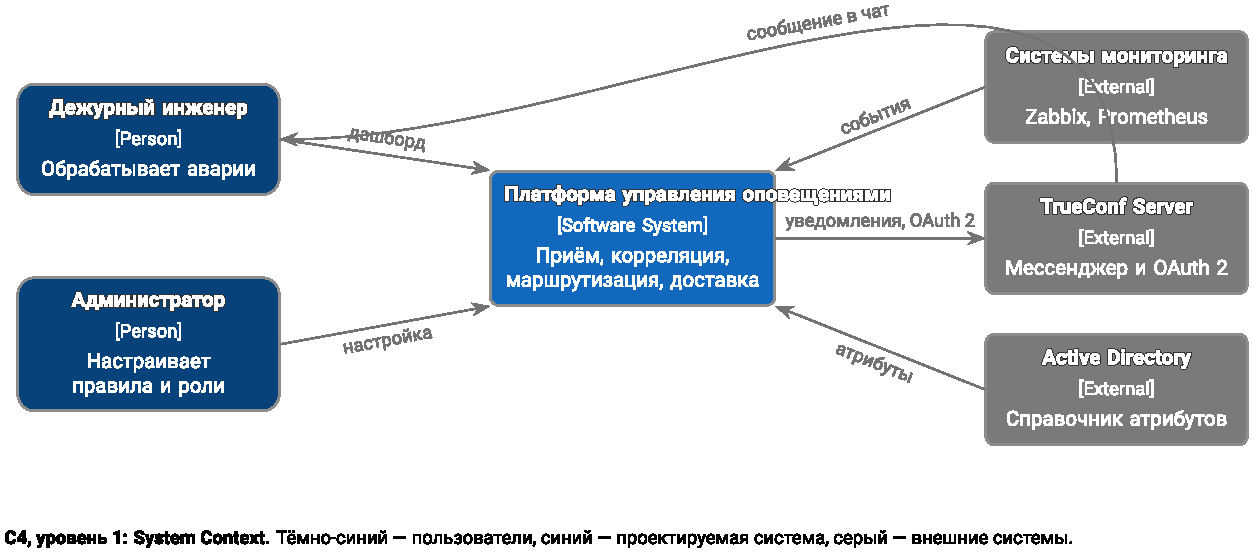
\includegraphics[width=\textwidth]{img/fig-context.pdf}
    \captionof{figure}{C4, уровень~1: контекст системы}
    \label{fig:context}
\end{figure}

Приём событий в целевой архитектуре вынесен в отдельный клиент-коннектор: на
каждый узел с системой мониторинга разворачивается свой экземпляр, который
приводит формат конкретного вендора к единой внутренней схеме и отправляет
результат платформе. Такое размещение решает три задачи: сетевую (система
мониторинга не должна иметь маршрута до ядра платформы, достаточно исходящего
соединения от коннектора), организационную (подключение новой площадки не
требует изменений в платформе) и эксплуатационную (сбой одного коннектора
изолирован в пределах своего узла).

Различие текущего и целевого размещения показано на
рисунке~\ref{fig:connector}. Оно затрагивает только упаковку и развёртывание:
адаптер источника~--- это реализация одного из двух интерфейсов, и один и тот
же код работает в обоих вариантах.

\begin{figure}[H]
    \centering
    \begin{minipage}[t]{0.48\textwidth}
        \centering
        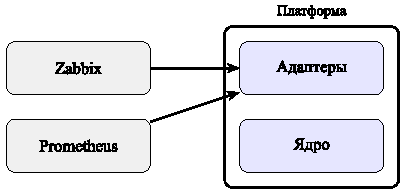
\includegraphics[width=0.82\textwidth]{img/fig-connector-asis.pdf}
        \\[0.3cm]
        {\footnotesize а)~текущая реализация пилота}
    \end{minipage}\hfill
    \begin{minipage}[t]{0.48\textwidth}
        \centering
        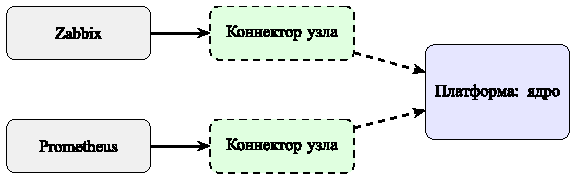
\includegraphics[width=\textwidth]{img/fig-connector-tobe.pdf}
        \\[0.3cm]
        {\footnotesize б)~целевая схема: коннектор на каждом узле}
    \end{minipage}
    \captionof{figure}{Размещение приёма событий: текущая реализация и целевая схема}
    \label{fig:connector}
\end{figure}

\subsection{Уровень 2: Containers}
Исполняемые единицы решения приведены на рисунке~\ref{fig:components}. Каждый
контейнер~--- это отдельный процесс или хранилище, разворачиваемое и
масштабируемое независимо; в скобках указана технология реализации. Хранилище и
ИИ-обработчик вынесены в сторону от основной цепочки, поскольку не лежат на
критическом пути доставки.

Граница «коннектор~--- платформа» реализована как контракт, а не как способ
запуска: адаптер источника~--- это реализация одного из двух интерфейсов
(источник вызывает нас по webhook либо мы опрашиваем источник), поэтому один и
тот же адаптер работает и в составе платформы, и как отдельный процесс на узле
мониторинга. В текущей реализации пилота адаптеры Alertmanager и Zabbix
выполняются внутри процесса платформы~--- это упрощает стенд, где все системы
мониторинга находятся на одном узле; целевая схема развёртывания~--- отдельный
клиент-коннектор на каждый узел, как показано на
рисунке~\ref{fig:context}. Изменение затрагивает только развёртывание:
контракты сообщений и код адаптеров остаются прежними.

\begin{landscape}
\begin{figure}[H]
    \centering
    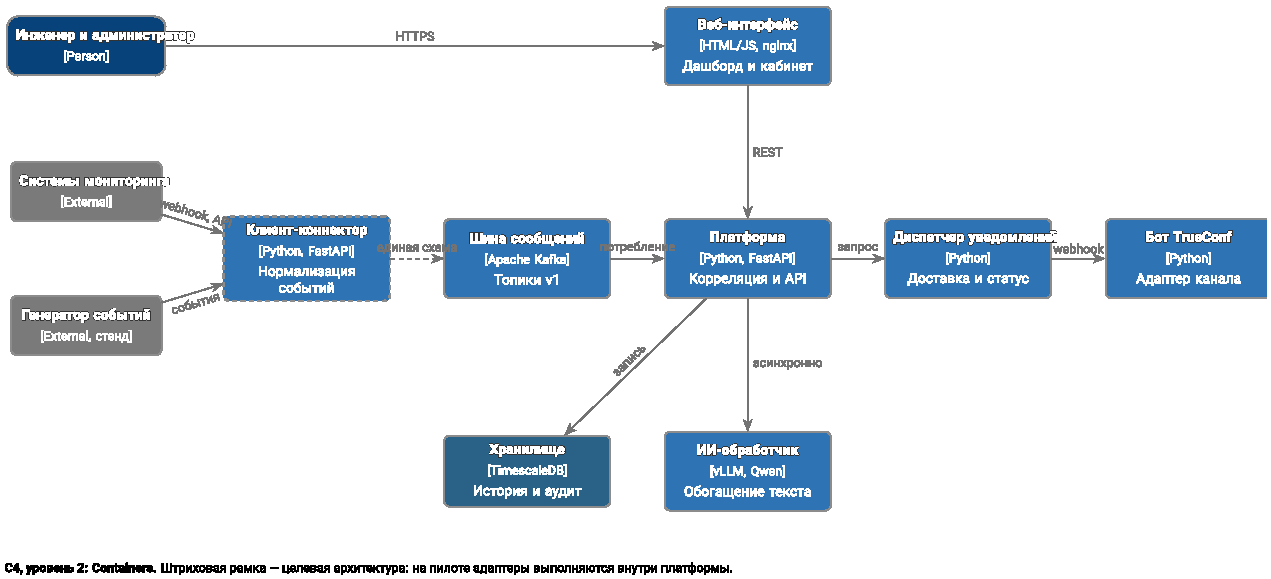
\includegraphics[width=\linewidth]{img/fig-components.pdf}
    \captionof{figure}{C4, уровень~2: контейнеры решения}
    \label{fig:components}
\end{figure}
\end{landscape}

\subsection{Уровень 3: Components}
Внутреннее устройство контейнера «Платформа» приведено на
рисунке~\ref{fig:c4component}. Компоненты соответствуют модулям репозитория:
приём и нормализация, фильтрация, корреляция, маршрутизация, \abbr{API} запросов,
идентификация и клиент ИИ. Клиент ИИ~--- единственный
компонент, обращающийся к модели: второго пути вызова в коде нет, что делает
контроль периметра и тайм-аутов проверяемым.

\begin{figure}[H]
    \centering
    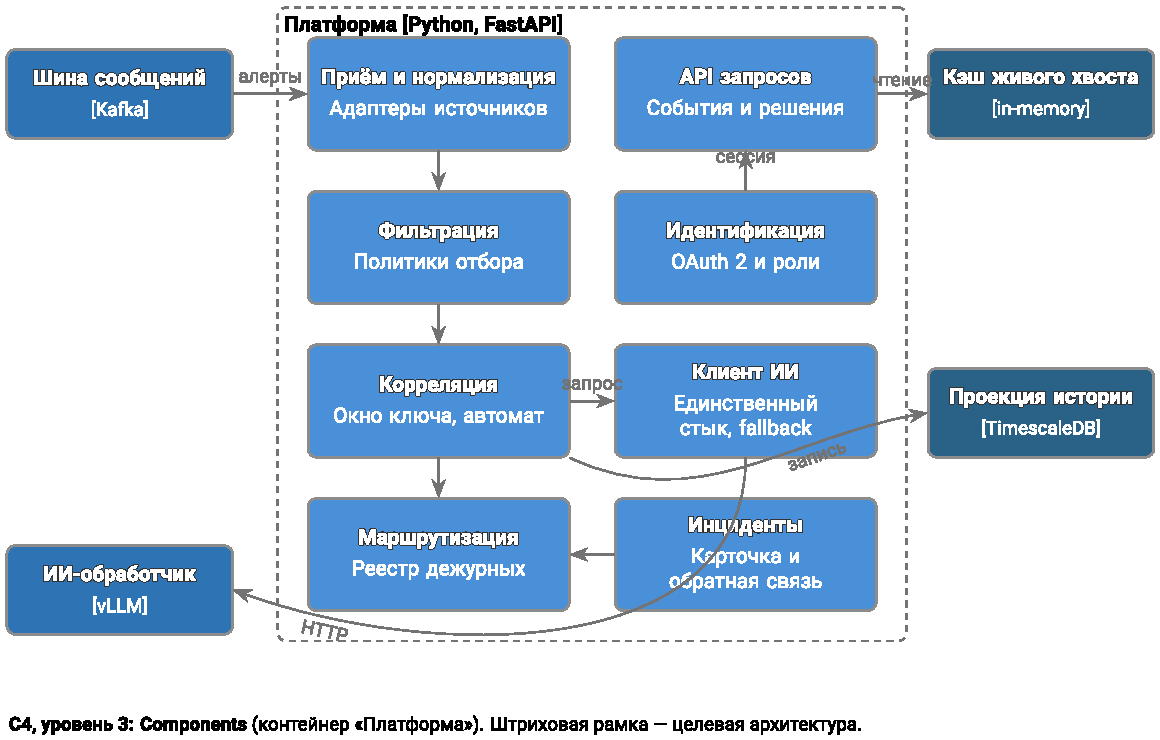
\includegraphics[width=\textwidth]{img/fig-c4component.pdf}
    \captionof{figure}{C4, уровень~3: компоненты контейнера «Платформа»}
    \label{fig:c4component}
\end{figure}

\subsection{Динамическое представление}
Путь одного алерта и точки принятия решений приведены на
рисунке~\ref{fig:flow}. Пунктиром показан ИИ-контур: он ответвляется от
основного пути после того, как детерминированное решение уже принято, и
поэтому не может задержать доставку.

\begin{figure}[H]
    \centering
    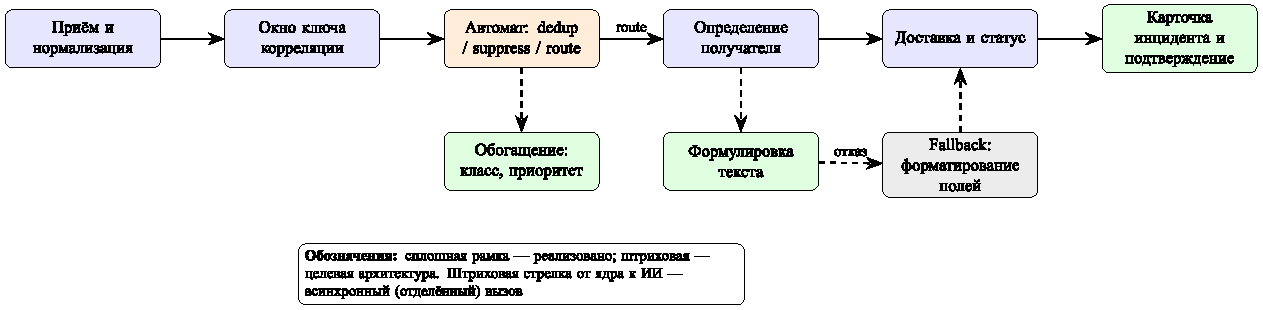
\includegraphics[width=\textwidth]{img/fig-flow.pdf}
    \captionof{figure}{Динамическое представление: путь алерта и точки принятия решений}
    \label{fig:flow}
\end{figure}

Полная матрица трассировки требований заказчика на архитектурные решения
(\reqAR{01}\,--\,\reqAR{17}) приведена в приложении~\ref{app:traceability}.

\section{Компоненты решения}
Решение развёртывается как набор независимых стеков, каждый со своей сетью и
томами; зоны ответственности приведены в таблице~\ref{tab:components}.

\begin{table}[H]
\centering
\caption{Компоненты решения}
\label{tab:components}
\resizebox{\textwidth}{!}{%
\begin{tabular}{|p{3.2cm}|p{7.5cm}|p{4.5cm}|}
\hline
\rowcolor{edtdark} \hcell{Компонент} & \hcell{Зона ответственности} & \hcell{Технологии} \\ \hline
Клиент-коннектор & Экземпляр на каждый узел мониторинга: приём webhook или опрос \abbr{API} вендора, приведение к единой схеме & Python, FastAPI \\ \hline
Генератор событий & Синтетический поток разноформатных событий, оценка по триггерным правилам, публикация в шину & Python, Kafka \\ \hline
Шина сообщений & Версионированные топики событий, алертов, решений, ИИ-запросов и результатов; очередь ошибок & Apache Kafka \\ \hline
Платформа (ядро) & Нормализация, фильтрация, корреляция, принятие решений, \abbr{API} для интерфейса, идентификация & Python, FastAPI \\ \hline
ИИ-контур & Семантическая обработка алертов: карантин, приоритизация, саммаризация, объяснение решений & vLLM, Qwen \\ \hline
Хранилище & Гипертаблицы истории событий, алертов и решений ИИ с политиками retention; реляционные таблицы личностей, ролей и связей & TimescaleDB \\ \hline
Веб-интерфейс & Дашборд администратора и личный кабинет; обратный прокси к \abbr{API} платформы & HTML/JS, nginx \\ \hline
Уведомления & Диспетчер доставки: чтение запросов на уведомление, отправка, фиксация статуса & Python, Kafka \\ \hline
Бот TrueConf & Адаптер обязательного канала доставки: приём запроса и отправка сообщения в личный чат & Python, TrueConf Chatbot \abbr{API} \\ \hline
Системы мониторинга & Реальные источники алертов пилота & Zabbix, Prometheus \\ \hline
Каталог AD & Номинальный справочник атрибутов (подразделение, команда) без роли в аутентификации & Samba AD DC \\ \hline
\end{tabular}%
}
\end{table}

\section{Используемые технологии}
% Обоснование выбора стека.


\chapter{Техническая реализация решения}

\section{Приём и нормализация событий}
Ингест реализован как точка расширения, а не как ветвление по названию
вендора. Определены два интерфейса подключения источника:

\begin{enumerate}[а)]
    \item источник вызывает платформу~--- webhook по адресу вида
          \texttt{/v1/integrations/<slug>/webhook}; маршрут находит адаптер,
          зарегистрированный на данный \texttt{slug}, и передаёт ему тело
          запроса целиком;
    \item платформа вызывает источник~--- адаптер реализуется как
          асинхронный итератор, который ядро опрашивает самостоятельно.
\end{enumerate}

По умолчанию подключены адаптеры Alertmanager~\cite{prometheus} и
Zabbix~\cite{zabbix}. Формат полезной
нагрузки полностью принадлежит адаптеру: Alertmanager присылает массив
объектов, Zabbix~--- плоский объект; маршрут о различии не знает.
Некорректная нагрузка приводит к отказу с кодом~422, а попытка зарегистрировать
два адаптера на один \texttt{slug} обнаруживается при запуске, а не молча
затеняет один другим. Дополнительно по расписанию выполняется сверка открытых
проблем через \abbr{API} Zabbix: webhook~--- быстрый путь, опрос~--- восстановление
пропущенных за время недоступности событий.

Внутренняя схема события намеренно минимальна и открыта: обязательны только
источник и статус, время подставляется при отсутствии, а любые дополнительные
поля вендора сохраняются как есть. Это позволяет подключить новый источник или
добавить производные признаки без миграции схемы. Схема алерта, напротив,
строгая: правило, критичность, метрика и порог обязательны, так как на них
опирается корреляция.

\section{Детерминированное ядро корреляции}
Каждый принятый алерт проходит потоковую обработку: постадийное преобразование
и последующая свёртка по ключу корреляции в пределах временного окна.
Ключ выбирается по первому доступному признаку: явный идентификатор корреляции,
затем сервис, затем пара «источник~--- метрика».

Политика свёртки реализована как конечный автомат на каждый ключ
(рисунок~\ref{fig:automaton}). Идентичностью сигнала считается тройка
«правило~--- метрика~--- источник»: два разных сигнала под одним ключом~---
это дополнительное свидетельство одной аварии, а не повтор.

\begin{figure}[H]
    \centering
    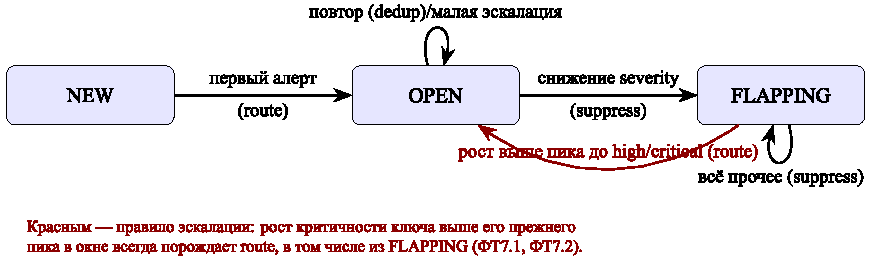
\includegraphics[width=0.95\textwidth]{img/fig-automaton.pdf}
    \captionof{figure}{Автомат корреляции: состояния ключа и принимаемые решения}
    \label{fig:automaton}
\end{figure}

Состояние не хранится как изменяемое поле: оно выводится проигрыванием всего
окна ключа при каждом вызове. Благодаря этому свёртка остаётся чистой функцией
от пары «ключ~--- окно», а признак нестабильности не может рассинхронизироваться
с историей. Неизвестная метка критичности не выводит ключ из обработки, а
трактуется как \texttt{warning}~--- один нестандартный вендорский ярлык не должен
ломать обработку.

Каждое принятое решение публикуется в топик решений и доступно через \abbr{API}, то
есть является наблюдаемым артефактом, а не внутренним состоянием.

\section{Маршрутизация и доставка}
Решение типа «маршрутизировать» преобразуется в запрос на уведомление:
реестр маршрутизации отображает «сервис~--- команда~--- дежурный~--- адрес
доставки». Идентификатор инцидента выводится детерминированно из ключа
корреляции, поэтому все алерты одной группы получают один идентификатор без
хранения состояния~--- это же обеспечивает дедупликацию на стороне диспетчера
после перезапуска.

Существенны два порядковых решения. Во-первых, получатель определяется
\emph{до} обращения к модели: алерт, у которого нет владельца, не должен
занимать слот \abbr{GPU}~--- при лавине событий это разница между очередью, которая
разбирается, и очередью, которая не разбирается. Во-вторых, отсутствующая или
повреждённая конфигурация маршрутизации деградирует до «никто не уведомлён» с
отражением в метрике, а не останавливает приём событий.

Доставка вынесена в отдельный диспетчер: он читает запросы на уведомление,
отправляет их и публикует результат~--- доставлено или не доставлено.
Обязательный канал TrueConf реализован как адаптер-бот, принимающий запрос по
webhook и отправляющий сообщение в личный чат.

\section{Веб-интерфейс}
Интерфейс разделён на две группы: управление (сводка, пользователи, матрица
ответственности, системы, маршрутизация, роли и права, политики \abbr{SLA},
интеграции, аудит) и мониторинг (инциденты, алерты, события, решения
корреляции). Он обращается к платформе через обратный прокси, поэтому браузер
работает с единственным origin~--- сессионная cookie аутентификации проходит
через прокси без настройки CORS.

Отдельно оговаривается честность отображения: разделы, не подключённые к
данным, показываются как макеты с явным баннером «Демонстрационные настройки»
(виден на рисунках~\ref{fig:ui-overview}--\ref{fig:ui-routing}), а не как
правдоподобные фиктивные данные. Тот же принцип действовал и на уровне
\abbr{API}: пока управление инцидентами не было реализовано, соответствующие
методы отвечали кодом~501, а не пустым списком, поскольку пустой список
неотличим от «сейчас ничего не происходит». Сейчас эти методы работают:
инцидент выводится из решений ядра, открывается только маршрутизацией (но не
дедупликацией и не подавлением) и подтверждается дежурным.

Главный экран~--- сводка эксплуатации (рисунок~\ref{fig:ui-overview}):
счётчики событий и алертов, распределение по критичности, состояние
компонентов платформы и блок «Требуют внимания». Состояние платформы, Kafka,
базы идентификаций и проекции алертов читается с backend в реальном времени;
операционные показатели на снимке~--- макет, о чём сообщает баннер.

\begin{figure}[H]
    \centering
    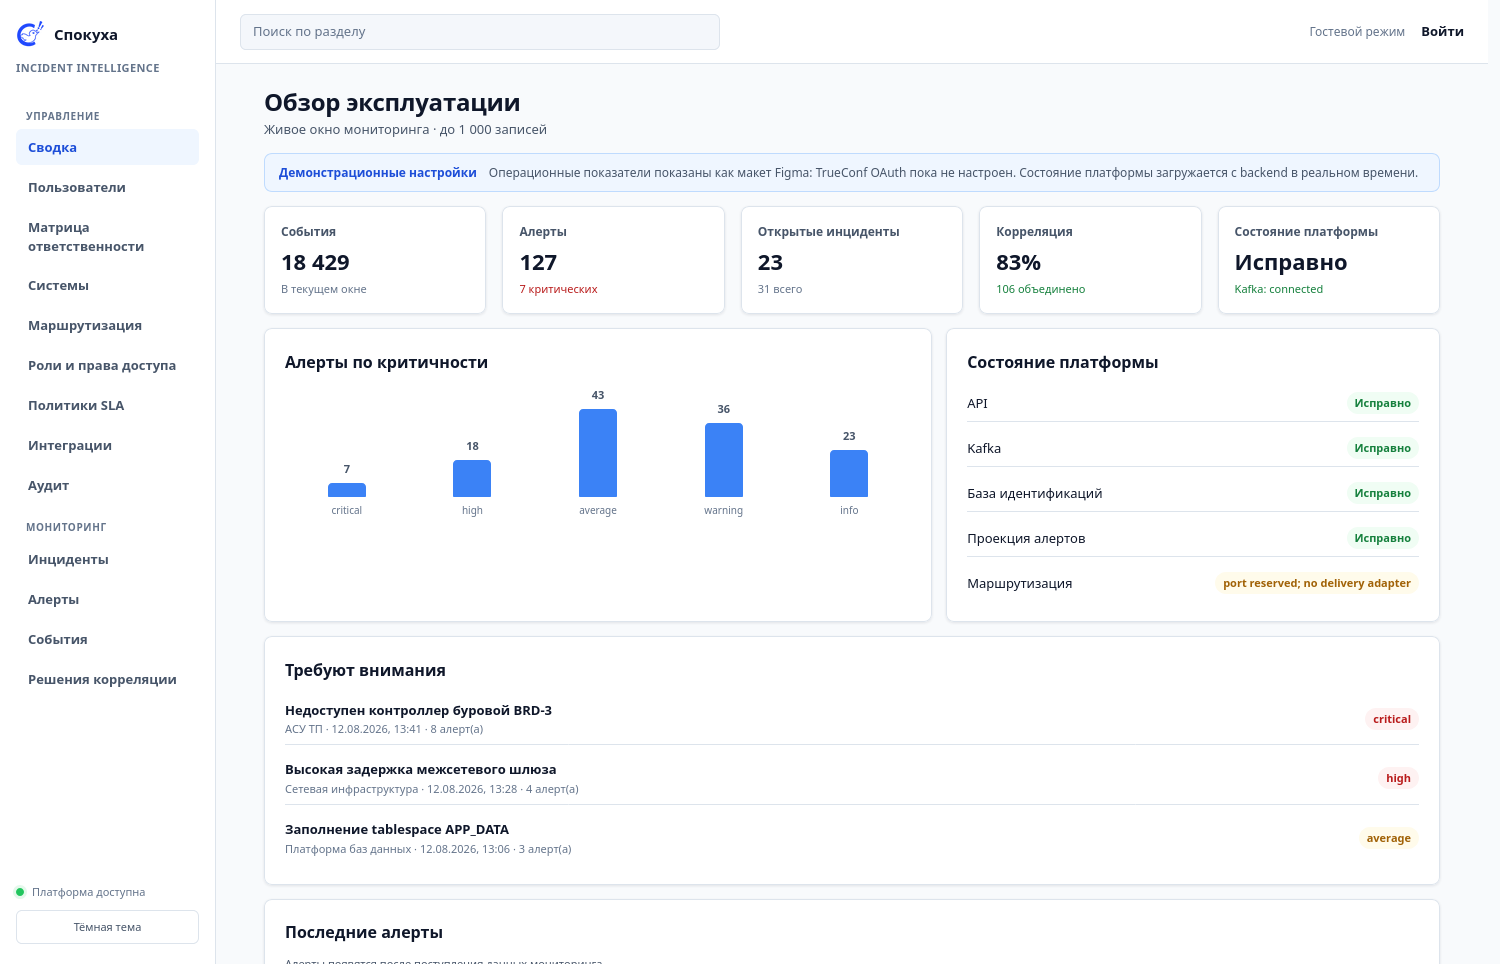
\includegraphics[width=\textwidth]{img/ui-overview.png}
    \captionof{figure}{Сводка эксплуатации: near-online дашборд}
    \label{fig:ui-overview}
\end{figure}

Раздел «Системы» (рисунок~\ref{fig:ui-systems}) объединяет каталог
контролируемых систем с их критичностью, владельцами и источником мониторинга
и живой перечень контуров платформы с их состоянием~--- включая honest-статусы
вида «port reserved; no delivery adapter» и «deferred; Alertmanager owns alert
lifecycle» для того, что ещё не подключено.

\begin{figure}[H]
    \centering
    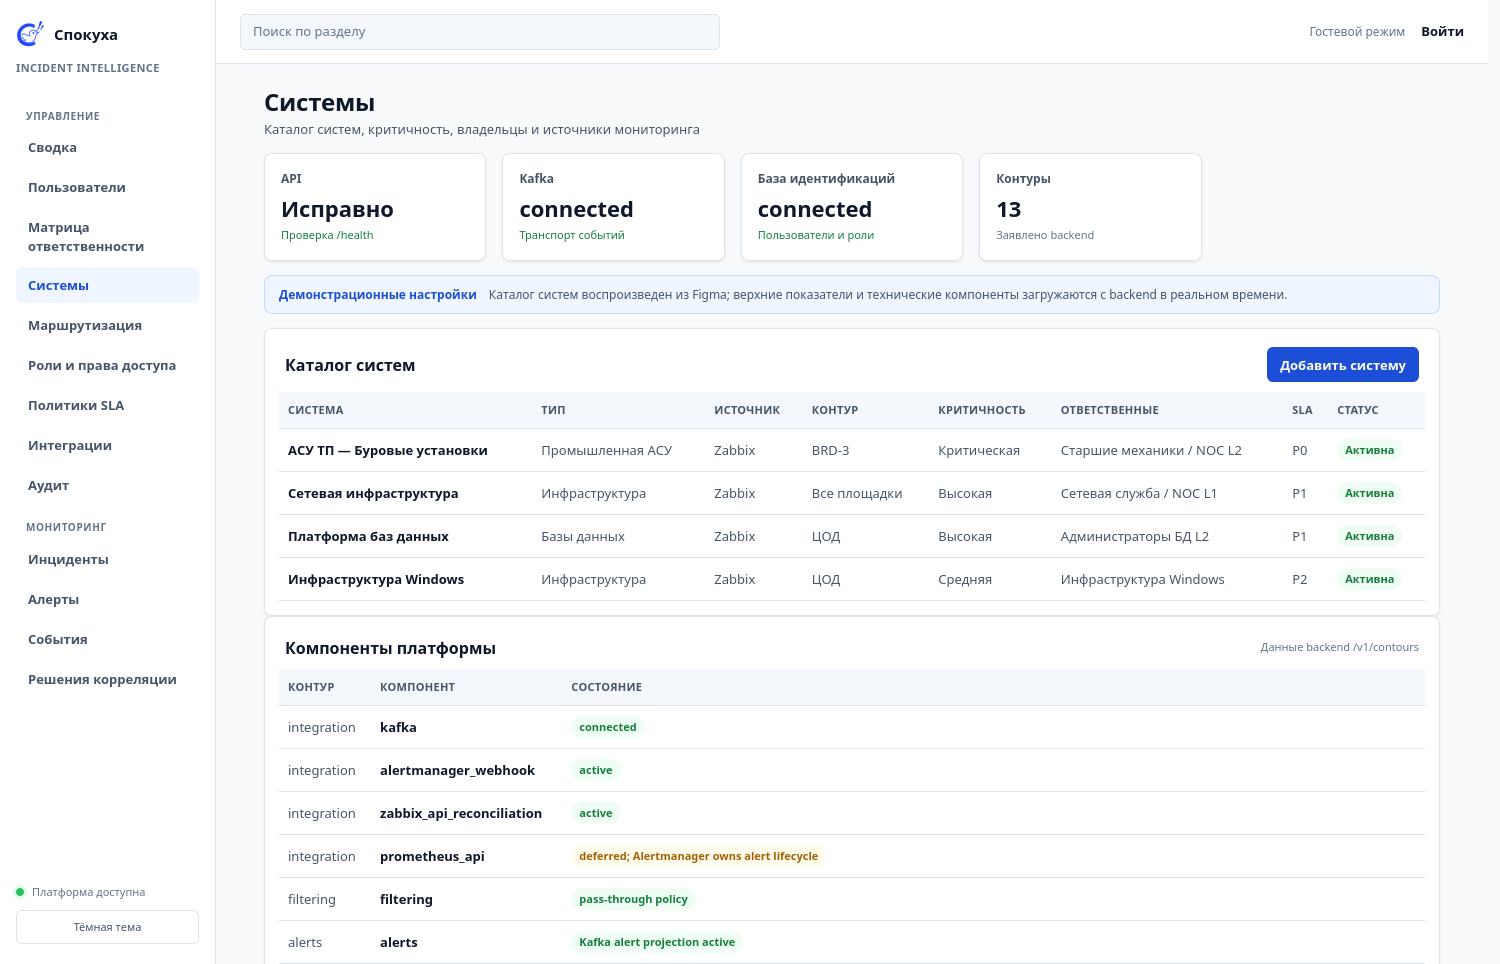
\includegraphics[width=\textwidth]{img/ui-systems.png}
    \captionof{figure}{Каталог систем и состояние контуров платформы}
    \label{fig:ui-systems}
\end{figure}

Административная часть представлена разделом маршрутизации
(рисунок~\ref{fig:ui-routing}): получатели и группы, правило маршрутизации по
критичности и источнику, условие отбора, первичный получатель и время
эскалации. Экран реализован по макету и подключается к административному \abbr{API}
на следующем этапе.

\begin{figure}[H]
    \centering
    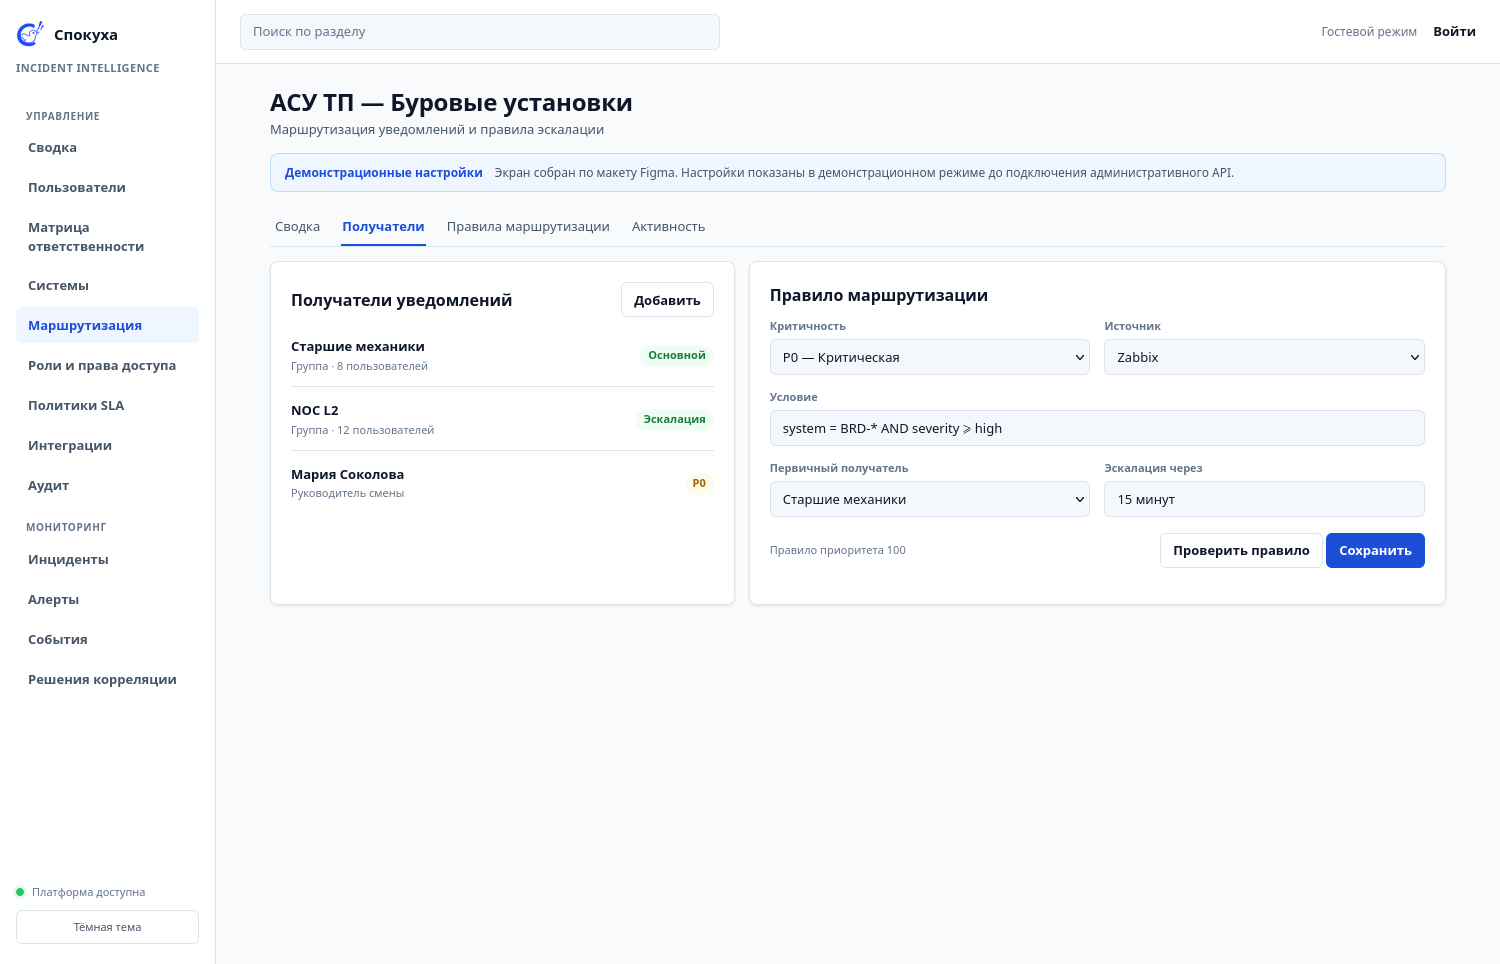
\includegraphics[width=\textwidth]{img/ui-routing.png}
    \captionof{figure}{Админ-панель: правила маршрутизации и эскалации}
    \label{fig:ui-routing}
\end{figure}

Для оперативной картины и для истории используются два разных хранилища:
ограниченный кэш «живого хвоста» в памяти отвечает на вопрос «что происходит
сейчас» (именно это опрашивает дашборд), а проекция в
TimescaleDB~\cite{timescaledb}~--- на вопросы истории и аудита. Растягивать кэш на обе задачи было бы ошибкой:
требования к ним противоположны.

\section{Идентификация и ролевая модель}
Аутентификация выполняется по OAuth~2 в потоке Authorization
Code~\cite{rfc6749} через TrueConf Server~\cite{trueconf}. Роли хранятся в таблице и засеяны значениями «наблюдатель», «инженер»,
«администратор»~--- добавление роли является вставкой записи, а не выпуском
новой версии кода. Первый вход любой учётной записи автоматически создаёт
личность с минимальной ролью, а роль повышает администратор.

Связь с Active Directory реализована как номинальный справочник атрибутов
(подразделение, команда) в собственной таблице платформы: платформа никогда не
создаёт и не изменяет учётные записи в реальном каталоге. Это прямое следствие
ограничения кейса и одновременно снятие зависимости от недоступного домена.

\section{Проверка качества обработки}
Для честной оценки фильтрации подготовлен воспроизводимый корпус событий.
Он генерируется декларативно: факты топологии (сервисы, узлы, зависимости,
команды, график дежурств, окна обслуживания) отделены от правил вывода
(транзитивное распространение отказа, порождение шума, понижение значимости в
окне обслуживания, разрешение адресата). Эталонная разметка не проставляется
руками, а выводится теми же правилами, поэтому не может разойтись с данными.
Корпус проверяется набором инвариантов до записи: например, смены дежурств
обязаны точно покрывать всё время корпуса без пропусков и наложений.

Текущий корпус: 1053 алерта (545 значимых, 508 шумовых), 8 инцидентов,
2~часа модельного времени. Оценка выполняется прогоном корпуса через реальный
конвейер в одном процессе~--- без Kafka, HTTP и развёртывания, за счёт
внедряемого источника времени. Результаты приведены в
таблице~\ref{tab:scoring}.

\begin{table}[H]
\centering
\caption{Качество обработки на эталонном корпусе (1053 алерта, 8 инцидентов)}
\label{tab:scoring}
\begin{tabular}{|l|c|c|c|c|}
\hline
\rowcolor{edtdark} \hcell{Вариант} & \hcell{Уведомлений} & \hcell{Снижение шума} & \hcell{Полнота} & \hcell{Точность} \\ \hline
Без фильтрации   & 1053 & 0,0\,\%  & 8/8 & 20,5\,\% \\ \hline
Автомат корреляции & 44 & 95,8\,\% & 8/8 & 31,8\,\% \\ \hline
\end{tabular}
\end{table}

Из 44~уведомлений варианта с корреляцией 14 адресованы верно, 13 ушли не
тому дежурному и 17 остались шумовыми (из них лишь одно~--- работа в окне
обслуживания). Для сравнения, базовая линия: 216 верных, 329 не тому адресату и
508 шумовых.

Полнота 8/8 достигнута не ослаблением фильтрации, а отдельным правилом
эскалации. Ранее второй инцидент, начавшийся, пока первый ещё каскадирует через
те же сервисы, попадал на уже открытый ключ и поглощался им: два одновременных
инцидента, делящих сервис, были неразличимы для корреляции по ключу сервиса,
и на корпусе терялся один инцидент из восьми. Автомат дополнен правилом: рост
критичности до high или critical \emph{выше пика, который ключ уже видел в
окне}, всегда порождает маршрутизацию~--- в том числе из состояния
нестабильности. Это прямое следствие запрета автоматически скрывать и подавлять
критичные алерты (\reqFT{7.1}, \reqFT{7.2}).

Правило остаётся экономным по построению: срабатывание привязано к росту
\emph{выше прежнего пика}, поэтому каждый уровень критичности порождает не
более одного уведомления на окно, а ключ, уже работающий на critical, повторно
не уведомляет. Цена восстановленной полноты измерена: восемь дополнительных
уведомлений (36~$\to$~44) и 0,8~процентного пункта снижения шума. Точность при
этом выросла с 27,8 до 31,8\,\%.

Оставшееся ограничение точности не устранено: уведомляется дежурный
\emph{сигнализирующего}, а не \emph{сломавшегося} сервиса, поэтому 13 из
44~уведомлений уходят не тому человеку. Это устраняется учётом первопричины и
данных \abbr{CMDB}.

Следует прямо оговорить границы измерения: один и тот же источник задаёт и шум,
и критерий шума, поэтому корпус~--- честный стенд для сравнения вариантов между
собой, но не доказательство эффективности на реальном трафике. Для последнего
нужны работающий приём из промышленного Zabbix и канал обратной связи от
инженеров.


\chapter{Конкурентоспособность и перспективы внедрения}

\section{Сравнение с существующими решениями}
Задача управления оповещениями решается тремя классами продуктов:
зарубежными SaaS-платформами реагирования на инциденты, встроенными средствами
самих систем мониторинга и российскими ITSM-платформами.
Сравнение по значимым для пилота критериям приведено в
таблице~\ref{tab:competitors}: \colorbox{cdone}{зелёным} отмечено соответствие
критерию, \colorbox{cpart}{жёлтым}~--- частичное, \colorbox{crisk}{красным}~---
несоответствие.

\begin{table}[H]
\centering
\caption{Сравнение классов решений}
\label{tab:competitors}
\resizebox{\textwidth}{!}{%
\begin{tabular}{|p{4cm}|p{3cm}|p{3.2cm}|p{3cm}|p{3.2cm}|}
\hline
\rowcolor{edtdark} \hcell{Критерий} & \hcell{Зарубежный SaaS} & \hcell{Средства мониторинга} & \hcell{ITSM-платформы} & \hcell{Настоящее решение} \\ \hline
Размещение данных & \srisk Внешнее облако & \sdone В контуре & \sdone В контуре & \sdone Полностью в контуре\\ \hline
Доступность в РФ & \spart Ограничена & \sdone Да & \sdone Да & \sdone Да\\ \hline
Несколько источников сразу & \sdone Да & \srisk Только свой & \spart Частично & \sdone Да, адаптерами\\ \hline
Корреляция между источниками & \sdone Да & \srisk Нет & \spart Ограниченно & \sdone Да\\ \hline
ИИ в контуре организации & \spart Обычно внешние \abbr{API} & \srisk Нет & \spart Редко & \sdone Да, локальный инференс\\ \hline
Доставка в TrueConf & \srisk Нет & \srisk Нет & \spart Через интеграцию & \sdone Штатный канал\\ \hline
Работа без реального AD & \spart Частично & --- & \srisk Обычно требуется & \sdone Да, OAuth~2 TrueConf\\ \hline
Стоимость владения & Подписка на пользователя & Входит в мониторинг & Лицензия и внедрение & Инфраструктура и сопровождение \\ \hline
\end{tabular}%
}
\end{table}

\section{Преимущества решения}
\begin{itemize}
    \item Полное размещение в корпоративном контуре, включая инференс языковой
          модели: исходящий доступ к внешним \abbr{API} моделей не требуется.
    \item Снижение шума подтверждено измерением на воспроизводимом корпусе, а
          не заявлено (таблица~\ref{tab:scoring}); вместе с ним измеряются и
          неудобные метрики~--- полнота и точность адресации.
    \item Работоспособность при отключённом ИИ: интеллектуальные функции
          являются надстройкой над детерминированным ядром, а не условием его
          работы.
    \item Настраиваемость вместо доработки: классификация, роли, правила
          маршрутизации и режимы автоматизации~--- конфигурация.
    \item Открытая точка расширения для источников: подключение новой системы
          мониторинга не затрагивает ядро.
\end{itemize}

\section{Ограничения пилота}
\label{sec:limits}
Честная оценка зрелости необходима для планирования внедрения:
\begin{itemize}
    \item состояние «инцидент решён» не выводится: публикуемого сигнала о
          восстановлении нет, а вывод его из «перестали приходить алерты» был бы
          догадкой, выданной за факт;
    \item часть разделов админ-панели существует в виде макетов и явно помечена
          как макеты;
    \item корреляция ведётся по ключу сервиса; одновременные инциденты на
          общем сервисе разделяются только при росте критичности до high или
          critical, при равной критичности они по-прежнему сливаются;
    \item маршрутизация опирается на владельца сигнализирующего сервиса, а не
          первопричины;
    \item масштабирование горизонтально возможно, но требует вынесения
          состояния ограничителя запросов и кэша во внешнее хранилище.
\end{itemize}

\section{План внедрения}
Внедрение планируется поэтапно, с управлением через флаги функциональности и
задокументированной процедурой отката:
\begin{enumerate}[1.]
    \item подключение первого источника в режиме наблюдения, дублирование
          критичных уведомлений существующим способом;
    \item включение корреляции и маршрутизации на ограниченном наборе сервисов,
          сверка адресатов с дежурными расписаниями;
    \item включение ИИ-функций в режимах shadow и suggest, накопление обратной
          связи;
    \item расширение периметра источников и подписчиков, отключение
          дублирования;
    \item переход отдельных функций в режим ограниченной автоматизации по
          достигнутым порогам уверенности.
\end{enumerate}


\chapter{Использование инструментов искусственного интеллекта}

\section{Место ИИ в архитектуре}
ИИ-контур подключён к основному потоку асинхронно. После того как
детерминированный путь обработки алерта завершён (сохранение, корреляция,
решение), запускается отделённая задача обогащения: запрос публикуется в топик
запросов, результат~--- в топик результатов. Разделение топиков сделано
заранее, чтобы масштабируемая группа обработчиков могла заменить встроенный
обработчик без изменения контракта.

Ключевое свойство контура~--- вызов модели не создаёт обратного давления на
приём алертов. Медленная или недоступная модель задерживает только собственный
результат.

\section{Реализованные ИИ-сценарии}
\begin{enumerate}[1.]
    \item \textbf{Обогащение алерта.} Один вызов модели с ограниченным JSON-ответом
          возвращает классификацию, приоритет, гипотезу первопричины,
          уверенность и объяснение. Значения классификации и приоритета
          ограничены объявленным словарём: ответ вне словаря отбрасывается и
          сохраняется только в объяснении, а не передаётся дальше как
          доверенный.
    \item \textbf{Формулировка уведомления.} Один вызов модели~\cite{qwen2024} формирует
          заголовок, приоритет и первый шаг проверки для сообщения дежурному
          (около 3,4\,с на используемом \abbr{GPU}). Любой отказ~--- недоступность
          модели, таймаут, некорректный JSON, приоритет вне словаря~--- приводит
          к детерминированному построению текста форматированием полей алерта.
          В полезной нагрузке уведомления фиксируется, каким путём получен
          текст, поэтому вопрос «как часто модель реально участвует» отвечается
          по данным, а не по логам.
\end{enumerate}

Обе функции реализованы через единственный сетевой стык с
моделью: второго способа вызвать модель в коде нет. Это делает контроль
периметра и таймаутов проверяемым.

\section{Соответствие требованиям БТ7}
Соответствие реализации требованиям к интеллектуальной обработке приведено в
таблице~\ref{tab:ai-requirements}. Здесь и далее состояние обозначено цветом:
\colorbox{cdone}{реализовано}, \colorbox{cpart}{реализовано частично},
\colorbox{cplan}{целевая архитектура}, \colorbox{cna}{неприменимо},
\colorbox{crisk}{первоочередной риск}.

\begin{longtable}{|p{1.4cm}|p{5.2cm}|p{7.4cm}|}
\caption{Соответствие требованиям БТ7}
\label{tab:ai-requirements} \\
\hline
\rowcolor{edtdark} \hcell{ID} & \hcell{Требование} & \hcell{Реализация и статус} \\ \hline
\endfirsthead
\multicolumn{3}{r}{\footnotesize Продолжение таблицы \thetable} \\
\hline
\rowcolor{edtdark} \hcell{ID} & \hcell{Требование} & \hcell{Реализация и статус} \\ \hline
\endhead
\endfoot
ПТ7.1 & Режимы off, shadow, suggest, assisted auto, full auto & \spart Режим задаётся флагом развёртывания; по умолчанию off. Реализованы off, shadow и suggest; режимы автоматизации зарезервированы контрактом и на пилоте не включаются\\ \hline
ПТ7.2 & Уровень автоматизации, порог уверенности, fallback & \sdone Уверенность возвращается по контракту и приводится к отрезку [0;\,1] независимо от ответа модели; fallback задан на каждом пути отказа\\ \hline
ПТ7.3 & ИИ не блокирует приём и доставку критичных алертов & \sdone Обогащение запускается после завершения детерминированного пути и выполняется как отделённая задача\\ \hline
ФТ7.1 & Дедупликация с сохранением истории & \spart Техническая дедупликация выполняется детерминированным автоматом с публикацией решения; смысловая дедупликация~--- задел ИИ-контура, автообъединение на пилоте отключено\\ \hline
ФТ7.2 & Карантин шумовых алертов, запрет автоподавления critical/high & \sdone Подавление выполняется только по правилу нестабильности сигнала; понижение критичности моделью не применяется автоматически\\ \hline
ФТ7.3 & Приоритизация & \sdone Приоритет предлагается моделью в словаре p1--p4; при отказе~--- детерминированное отображение критичности в приоритет\\ \hline
ФТ7.4 & Маршрутизация по каталогу, владельцам и дежурствам & \sdone Реализована детерминированно по реестру маршрутизации; при отсутствии владельца уведомление не отправляется и фиксируется как немаршрутизируемое\\ \hline
ФТ7.5 & Декомпозиция составных инцидентов & \splan На пилоте отключена в соответствии с требованием; предпосылка появилась~--- инцидент реализован как проекция решений ядра \\ \hline
ФТ7.6 & Объяснимость решения & \sdone Результат содержит объяснение, уверенность и признаки; версия политики корреляции фиксируется идентификатором политики\\ \hline
ФТ7.7 & Обратная связь пользователя & \spart Частично: подтверждение обработки инцидента реализовано, автор берётся из сессии; переопределение решения ИИ с указанием причины~--- нет \\ \hline
НФТ7.1 & Аудит решений ИИ & \sdone Решения пишутся в отдельную гипертаблицу с увеличенным сроком хранения (по умолчанию 400 дней против 90 у событий и алертов)\\ \hline
НФТ7.2 & Fallback на детерминированные правила & \sdone Обеспечен архитектурно: ядро не зависит от модели\\ \hline
НФТ7.3 & Задержка ИИ не задерживает critical & \sdone Обеспечено отделённым вызовом и ограничением числа одновременных обращений к модели\\ \hline
НФТ7.4 & Запрет передачи секретов и \abbr{ПДн}, недоверенный текст алерта & \sdone Инференс размещён в контуре; в модель передаются только технические поля алерта; ответ модели принимается только в пределах объявленного словаря\\ \hline
\end{longtable}

\section{ИИ в процессе разработки}
Инструменты на основе больших языковых моделей применялись при разработке для
генерации и рефакторинга кода, подготовки тестовых сценариев и документации.
Принятые ограничения: архитектурные решения и границы контуров определялись
разработчиками, весь сгенерированный код проходил ревью и покрывался тестами,
а формулировки требований и матрица трассировки поддерживались вручную.


\chapter{Инфраструктура решения}

\section{Топология развёртывания}
Решение развёртывается как набор независимых Docker Compose~\cite{docker} стеков: каждый со
своим именем проекта, собственной сетью и томами. Стеки поднимаются независимо,
за исключением случаев, когда один присоединяется к сети другого. Платформа
присоединяется к сетям генератора событий, Prometheus, Zabbix и TimescaleDB;
веб-интерфейс~--- к сети платформы.

Наружу публикуются только те порты, которые действительно нужны: база данных
host-порта не имеет вовсе и доступна исключительно платформе по внутренней
сети. Распределение портов пилотного стенда приведено в
таблице~\ref{tab:ports}.

\begin{table}[H]
\centering
\caption{Порты пилотного стенда}
\label{tab:ports}
\begin{tabular}{|l|l|l|}
\hline
\rowcolor{edtdark} \hcell{Порт} & \hcell{Стек} & \hcell{Назначение} \\ \hline
8080 & Zabbix & веб-интерфейс мониторинга \\ \hline
9090 / 9093 & Prometheus & мониторинг и Alertmanager \\ \hline
8090 & Генератор событий & приём событий (Kafka не публикуется) \\ \hline
8100 & Платформа & \abbr{API} \\ \hline
8091 & Веб-интерфейс & дашборд \\ \hline
8110 & Уведомления & диспетчер доставки \\ \hline
8120 & Бот TrueConf & приём запросов на доставку \\ \hline
80 / 443 / 4307 & TrueConf Server & мессенджер \\ \hline
8443 / 8543 & TLS-фронт & HTTPS для TrueConf и веб-интерфейса \\ \hline
--- & TimescaleDB & только внутренняя сеть \\ \hline
\end{tabular}
\end{table}

Отдельного пояснения требует размещение коннекторов. Целевая схема~---
экземпляр клиента-коннектора на каждом узле с системой мониторинга: он
устанавливается в сетевом сегменте этого узла и инициирует исходящее соединение
к платформе, поэтому системе мониторинга не требуется маршрут до ядра. На
пилотном стенде все системы мониторинга находятся на одном узле, и адаптеры
выполняются внутри процесса платформы; переход к распределённой схеме не
затрагивает контракты сообщений и код адаптеров, а только их упаковку и
размещение.

\section{Потребление ресурсов}
Приведённые ниже значения~--- не оценка, а замер работающего пилотного стенда:
виртуальная машина 16~vCPU, 62~ГБ ОЗУ, 133~ГБ диска и \abbr{GPU} Tesla~T4 (15~ГБ),
15~контейнеров, аптайм 5~суток. Замер снят в режиме ожидания (без нагрузочного
прогона), поэтому показывает базовое, а не пиковое потребление
(таблица~\ref{tab:resources}).

\begin{longtable}{|p{4.4cm}|p{1.8cm}|p{2.2cm}|p{6.2cm}|}
\caption{Замеренное потребление ресурсов пилотного стенда}
\label{tab:resources} \\
\hline
\rowcolor{edtdark} \hcell{Компонент} & \hcell{CPU} & \hcell{ОЗУ} & \hcell{Примечание} \\ \hline
\endfirsthead
\multicolumn{4}{r}{\footnotesize Продолжение таблицы \thetable} \\
\hline
\rowcolor{edtdark} \hcell{Компонент} & \hcell{CPU} & \hcell{ОЗУ} & \hcell{Примечание} \\ \hline
\endhead
\endfoot
Платформа (монолит) & 0,4\,\% & 65 МБ & Основная логика: приём, корреляция, \abbr{API} \\ \hline
Веб-интерфейс & $<0{,}1$\,\% & 13 МБ & Статика и обратный прокси \\ \hline
TimescaleDB & 0,8\,\% & 384 МБ & Растёт с объёмом истории \\ \hline
Kafka & 181\,\% & 1,2 ГБ & В простое занимает около 1,8~ядра~--- см. пояснение ниже \\ \hline
Генератор событий & 0,4\,\% & 40 МБ & Только на стенде \\ \hline
Инференс vLLM & 1,2\,\% & 4,0 ГБ & Плюс 13,6 из 15,4 ГБ видеопамяти под весами модели \\ \hline
TrueConf Server & 0,5\,\% & 1,25 ГБ & Внешняя система, обычно уже есть у заказчика \\ \hline
Контроллер домена & 0,2\,\% & 255 МБ & Синтетический справочник стенда \\ \hline
Zabbix (\abbr{СУБД}, сервер, веб, агент) & 1,1\,\% & 945 МБ & Источник событий, обычно уже есть \\ \hline
Prometheus & $<0{,}1$\,\% & 44 МБ & Источник событий и метрик \\ \hline
Сервис \abbr{CMDB} & 0,1\,\% & 33 МБ & Развёрнут на стенде, платформой пока не используется \\ \hline
TLS-фронт & $<0{,}1$\,\% & 16 МБ & Терминация \abbr{TLS} \\ \hline
\textbf{Итого} & \textbf{$\approx$\,1,9 ядра} & \textbf{$\approx$\,9 ГБ} & Диск: 38 ГБ образов, 2,2 ГБ томов, всего занято 74 ГБ \\ \hline
\end{longtable}

Из замера следуют три вывода, влияющие на выбор конфигурации.

Во-первых, \textbf{прикладные компоненты почти ничего не потребляют}: платформа,
интерфейс и диспетчер доставки вместе занимают менее 150~МБ ОЗУ и доли процента
процессора. Ограничением является не прикладной код, а инфраструктура под ним.

Во-вторых, \textbf{основной потребитель процессора~--- шина сообщений}: Kafka в
простое занимает около 1,8~ядра, то есть больше, чем все остальные контейнеры
вместе. Это конфигурация стенда с одним брокером и настройками по умолчанию;
для промышленной эксплуатации требуется отдельный узел и настройка, а не
соседство с прикладными сервисами.

В-третьих, \textbf{ИИ-контур ограничен видеопамятью, а не процессором}: модель
занимает 13,6 из 15,4~ГБ видеопамяти постоянно, независимо от нагрузки, при
загрузке \abbr{GPU} 0\,\% в простое. Это и есть причина размещать инференс отдельно:
он масштабируется другой величиной (видеопамять и число одновременных запросов),
чем всё остальное.

\section{Целевая конфигурация}
Схема развёртывания приведена на рисунке~\ref{fig:deploy}: виртуальные машины,
контейнеры внутри них и направление роста каждого узла.

\begin{figure}[H]
    \centering
    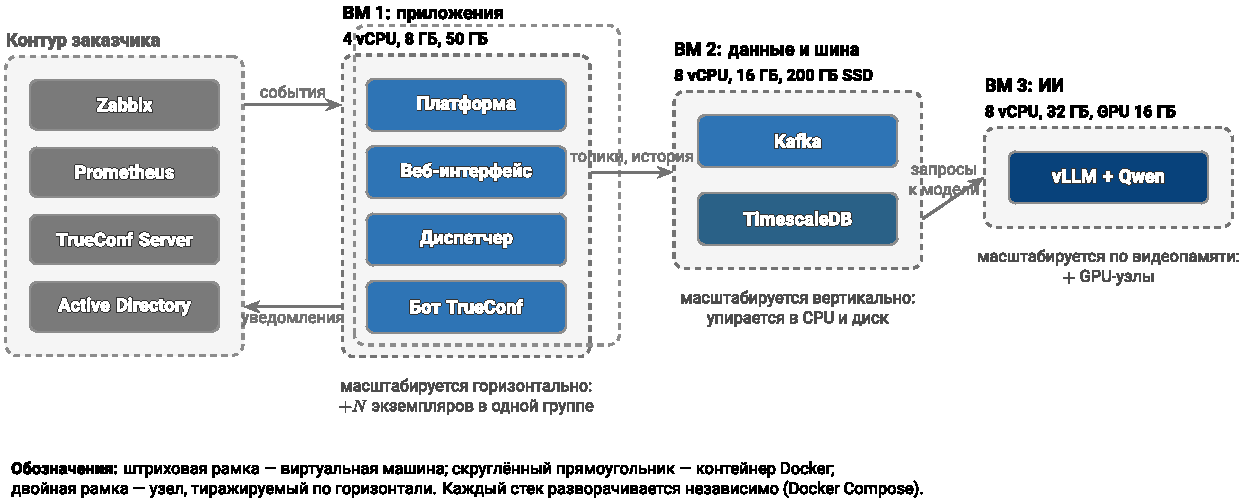
\includegraphics[width=\textwidth]{img/fig-deploy.pdf}
    \captionof{figure}{Развёртывание и масштабирование: узлы, контейнеры, направление роста}
    \label{fig:deploy}
\end{figure}

Развёртывание планируется раздельным: монолиты платформы отдельно, ИИ-сервисы
отдельно, данные и шина отдельно. Такое разделение отражает разные профили
потребления из предыдущего раздела и разные требования к масштабированию.
Целевые конфигурации приведены в таблице~\ref{tab:sizing}.

\begin{longtable}{|p{3.4cm}|p{4.2cm}|p{3.4cm}|p{4cm}|}
\caption{Целевая конфигурация узлов}
\label{tab:sizing} \\
\hline
\rowcolor{edtdark} \hcell{Узел} & \hcell{Состав} & \hcell{Конфигурация} & \hcell{Чем ограничен} \\ \hline
\endfirsthead
\multicolumn{4}{r}{\footnotesize Продолжение таблицы \thetable} \\
\hline
\rowcolor{edtdark} \hcell{Узел} & \hcell{Состав} & \hcell{Конфигурация} & \hcell{Чем ограничен} \\ \hline
\endhead
\endfoot
Приложения & Платформа, веб-интерфейс, диспетчер доставки, бот, коннекторы & 4 vCPU, 8 ГБ ОЗУ, 50 ГБ & Числом экземпляров, не ресурсами; запас $\approx$\,50-кратный к замеру \\ \hline
Данные и шина & Kafka, TimescaleDB & 8 vCPU, 16 ГБ ОЗУ, 200 ГБ SSD & Процессором (шина) и диском (история); растёт с retention \\ \hline
ИИ & vLLM, будущие обработчики & 8 vCPU, 32 ГБ ОЗУ, \abbr{GPU} 16~ГБ, 100 ГБ & Видеопамятью и числом одновременных запросов \\ \hline
Интеграции & Zabbix, Prometheus, каталог, TrueConf & Ресурсы заказчика & Обычно уже развёрнуто; в расчёт затрат не включается \\ \hline
\end{longtable}

Разделение даёт три эксплуатационных следствия: прикладной узел можно
перезапускать и масштабировать, не трогая шину и историю; отключение или
перезагрузка ИИ-узла не влияет на приём и доставку (это же свойство проверено
тестами); а \abbr{GPU}~--- самый дорогой ресурс~--- выделяется только под инференс и
не простаивает в составе прикладного узла.

\section{Развёртывание}
Конфигурация разделена на два уровня: версионируемый файл флагов (версии
образов, порты, тайм-ауты, режимы) и приватный файл секретов, который
генерируется на целевом узле и никогда не попадает в репозиторий и не
перезаписывается при развёртывании. Развёртывание выполняется скриптом:
синхронизация стека, запуск, проверка состояния контейнеров и обращение к
адресу проверки работоспособности с однозначным результатом.

\section{Модель масштабирования}
Масштабирование выполняется добавлением экземпляров платформы и обработчиков:
это участники одной группы потребителей Kafka, разделяющие партиции.
Kafka при этом не масштабируется~--- она является буфером, а не узким местом;
узкими местами являются \abbr{СУБД} и инференс модели, и их масштабирование~---
отдельное решение.

Принятый компромисс формулируется явно: это масштабирование виртуальными
машинами, а не оркестратором. Узел является одновременно единицей масштаба и
единицей отказа: при потере узла его контейнеры остаются недоступны до ручного
переразвёртывания. Такое решение даёт рост пропускной способности, но не
отказоустойчивость; при появлении требования к непрерывности потребуется
оркестратор. До запуска второго экземпляра платформы требуется вынести во
внешнее хранилище состояние ограничителя запросов и кэш живого хвоста.

\section{Наблюдаемость}
Состав наблюдаемости и подход к дежурству опираются на практики эксплуатации
крупных production-систем~\cite{beyer2016, beyer2018}.
Каждый стек публикует метрики в формате Prometheus и предоставляет адрес
проверки работоспособности, включающий состояние подключения к Kafka и к базе.
Метрики уведомлений размечены исходом и способом формирования текста, что
позволяет отслеживать долю немаршрутизируемых алертов и фактический вклад
модели.


\chapter{Информационная безопасность}

\section{Подход и границы моделирования}
Модель угроз описывает, \emph{кто} и \emph{каким способом} может нарушить
работу платформы, и служит основанием для выбора защитных мер. Она отвечает на
вопрос «что может пойти не так», тогда как оценка ущерба и приоритет
устранения~--- предмет реестра рисков и вынесены в
раздел~\ref{sec:ibgap}. Угроза является входом для риска: перечень угроз
первичен, приоритизация~--- вторична.

Границы моделирования: рассматривается платформа управления оповещениями и её
интерфейсы с внешними системами. Сами системы мониторинга, мессенджер и
каталог считаются внешними и защищаются собственными средствами; в модели они
присутствуют как источники недоверенных данных и как объекты, доступ к которым
может быть использован против платформы.

Объектами защиты являются: достоверность и целостность событий; доступность
критического пути доставки; целостность решений о критичности и адресате;
разграничение доступа к данным мониторинга; доказуемость действий (аудит);
конфиденциальность секретов и технических идентификаторов.

Классификация угроз для интеллектуальных компонентов опирается на
OWASP~Top~10 для приложений с большими языковыми
моделями~\cite{owaspllm2025} и рамочную модель управления рисками
ИИ~\cite{nistairmf}; требования к веб-контуру~--- на
OWASP~ASVS~\cite{owaspasvs}. Для промышленной эксплуатации на объектах
критической информационной инфраструктуры дополнительно применяются
187-ФЗ~\cite{fz187} и приказ ФСТЭК России №~239~\cite{fstek239}, а система
менеджмента ИБ~--- ГОСТ~Р~ИСО/МЭК~27001-2021~\cite{gost27001}.

\section{Модель нарушителя}
Категории нарушителей и их возможности приведены в
таблице~\ref{tab:intruder}. Категории упорядочены по возрастанию возможностей;
нарушитель более высокой категории обладает всеми возможностями предыдущих.

\begin{longtable}{|p{1.1cm}|p{4.0cm}|p{5.2cm}|p{4.6cm}|}
\caption{Категории нарушителей}
\label{tab:intruder} \\
\hline
\rowcolor{edtdark} \hcell{Код} & \hcell{Нарушитель} & \hcell{Возможности} & \hcell{Мотивация} \\ \hline
\endfirsthead
\multicolumn{4}{r}{\footnotesize Продолжение таблицы \thetable} \\
\hline
\rowcolor{edtdark} \hcell{Код} & \hcell{Нарушитель} & \hcell{Возможности} & \hcell{Мотивация} \\ \hline
\endhead
\endfoot
Н1 & Внешний, без доступа к корпоративной сети & Обращение к опубликованным точкам входа: веб-интерфейс, TLS-фронт & Отказ в обслуживании, разведка инфраструктуры \\ \hline
Н2 & Внешний, с доступом к сегменту мониторинга & Отправка произвольных сообщений на точки приёма webhook, наблюдение внутреннего трафика сегмента & Подделка или сокрытие аварий \\ \hline
Н3 & Внутренний пользователь платформы (наблюдатель, инженер) & Аутентифицированный доступ к данным мониторинга в пределах своей роли & Превышение прав, доступ к чужим объектам \\ \hline
Н4 & Внутренний администратор платформы & Изменение ролей, правил маршрутизации, режимов ИИ и подписок & Сокрытие собственных действий, злоупотребление правами \\ \hline
Н5 & Администратор инфраструктуры (узел, контейнеры) & Доступ к файлам конфигурации, секретам, томам и журналам & Доступ к данным в обход прикладных проверок \\ \hline
Н6 & Поставщик программных компонентов & Внесение изменений в зависимости, образы и веса модели до их попадания в контур & Закрепление в контуре, скрытая функциональность \\ \hline
Н7 & Автор текста алерта (косвенный нарушитель) & Формирование содержимого события, попадающего в модель как данные & Манипуляция решением интеллектуального контура \\ \hline
\end{longtable}

Нарушитель Н7 выделен отдельно, поскольку он не имеет никакого доступа к
системе: его единственный инструмент~--- содержимое поля алерта, которое
платформа обязана принять. Именно эта категория делает обязательным правило
«текст алерта~--- недоверенные данные».

\section{Перечень угроз}
Угрозы приведены в таблице~\ref{tab:threats} в форме «угроза~--- вектор
реализации~--- меры противодействия». Столбец мер перечисляет полный требуемый
набор, а столбец состояния показывает, какая его часть реализована:
нейтрализована, нейтрализована частично, не нейтрализована либо неактуальна для
текущей архитектуры с указанием причины. Развёрнутое описание мер по контурам
приведено в разделах~\ref{sec:ibinput}--\ref{sec:ibmonitor}.

\begin{landscape}
\begin{longtable}{|p{1.0cm}|p{1.0cm}|p{5.0cm}|p{3.8cm}|p{6.0cm}|p{4.2cm}|}
\caption{Перечень угроз безопасности информации}
\label{tab:threats} \\
\hline
\rowcolor{edtdark} \hcell{Код} & \hcell{Наруш.} & \hcell{Вектор реализации} & \hcell{Последствие} & \hcell{Меры противодействия} & \hcell{Состояние} \\ \hline
\endfirsthead
\multicolumn{6}{r}{\footnotesize Продолжение таблицы \thetable} \\
\hline
\rowcolor{edtdark} \hcell{Код} & \hcell{Наруш.} & \hcell{Вектор реализации} & \hcell{Последствие} & \hcell{Меры противодействия} & \hcell{Состояние} \\ \hline
\endhead
\endfoot
У-01 & Н2 & Отправка сфабрикованных событий на неаутентифицированную точку приёма webhook & Ложные аварии, отвлечение дежурных, маскировка реальной аварии & Отдельная идентичность источника, взаимная аутентификация или подпись запроса, allowlist адресов, аудит подключений & \srisk Не нейтрализована: аутентификация источника не реализована \\ \hline
У-02 & Н2 & Массовая отправка событий (лавина) с целью исчерпания обработки & Задержка или потеря критичных уведомлений & Ограничение частоты на входе, буферизация в шине, подавление нестабильных ключей, приоритетные очереди для critical, квоты по источникам & \spart Частично: ограничение частоты и буферизация есть, приоритетных очередей нет \\ \hline
У-03 & Н2 & Повторная отправка ранее принятого события & Дублирование инцидентов, повторные уведомления & Детерминированные идентификаторы сообщения и корреляции, дедупликация в автомате, проверка идемпотентности на приёме & \spart Частично: идентификаторы детерминированы, отдельной проверки идемпотентности приёма нет \\ \hline
У-04 & Н2 & Передача некорректной или вредоносной структуры данных вендора & Отказ обработчика, порча внутреннего состояния & Строгая схема входных данных, отказ 422 вместо интерпретации, изоляция адаптеров, запрет двух адаптеров на один идентификатор & \sdone Нейтрализована \\ \hline
У-05 & Н1 & Перебор и автоматизированные обращения к API и точкам аутентификации & Отказ в обслуживании, подбор учётных данных & Раздельные политики ограничения частоты для webhook и API, TLS на периметре, WAF и защита от перебора & \spart Частично: ограничение частоты по префиксам есть, WAF отсутствует \\ \hline
У-06 & Н7 & Внедрение инструкций в текст алерта, попадающий в модель & Изменение классификации, приоритета или адресата & Разделение инструкции и данных в запросе, приём ответа только в пределах словаря, отсутствие полномочий у модели, критичные решения вне модели & \sdone Нейтрализована \\ \hline
У-07 & Н7 & Формирование текста, вызывающего аномально долгую обработку моделью & Задержка обогащения, исчерпание слотов GPU & Отделённый вызов, тайм-аут, ограничение числа параллельных обращений, разрешение получателя до обращения к модели & \sdone Нейтрализована \\ \hline
У-08 & --- & Недоступность или деградация модели & Остановка обработки при синхронной зависимости & Детерминированное ядро, fire-and-forget вызов, fallback на форматирование полей, флаг отключения контура & \sdone Нейтрализована архитектурно, подтверждено тестами \\ \hline
У-09 & Н3 & Обращение к данным и объектам за пределами своей роли & Раскрытие сведений об инфраструктуре и авариях & Аутентификация для всех разделов мониторинга, ролевая модель, объектная авторизация по владельцу и команде & \spart Частично: ролевая модель есть, объектной авторизации нет \\ \hline
У-10 & Н1, Н3 & Кража сессионного токена (перехват, межсайтовый сценарий) & Действия от имени пользователя & TLS, httponly-cookie, передача токена во фрагменте URL, строгий список адресов возврата, второй фактор, ограничение времени жизни сессии & \spart Частично: второго фактора нет \\ \hline
У-11 & Н4 & Изменение правил маршрутизации или подписок, чтобы не уведомлять о конкретной аварии & Сокрытие инцидента & Журналирование всех изменений правил и подписок, обязательные подписки на critical, разделение полномочий, оповещение о смене режима ИИ & \spart Частично: журналирование есть, неизменяемого хранилища аудита нет \\ \hline
У-12 & Н4, Н5 & Изменение или удаление записей аудита & Невозможность разбора инцидента, отрицание действий & Отдельное хранилище аудита в режиме только на дозапись, ограниченный круг пишущих компонентов, увеличенный срок хранения & \spart Частично: увеличенный срок хранения решений, режим только на дозапись не реализован \\ \hline
У-13 & Н5 & Извлечение секретов из файлов конфигурации, переменных окружения или журналов & Доступ к базе, мессенджеру, API мониторинга & Централизованное хранилище секретов, внедрение в среду выполнения, ротация, маскирование в журналах, автоматическая проверка на секреты & \spart Частично: секреты вне репозитория, хранилища и ротации нет \\ \hline
У-14 & Н5 & Горизонтальное перемещение между контейнерами и сетями стенда & Расширение зоны поражения & Сегментация сетей, запуск не от суперпользователя, запрет привилегированного режима, ограничение возможностей ядра, файловая система только для чтения & \spart Частично: сегментация есть, ограничения привилегий не применены \\ \hline
У-15 & Н5 & Прямое обращение к хранилищу в обход прикладных проверок & Чтение и изменение истории и ролей & Отсутствие публикуемого порта у СУБД, раздельные сервисные учётные записи с минимальными правами, шифрование и резервное копирование & \spart Частично: порт не публикуется, раздельных учётных записей нет \\ \hline
У-16 & Н6 & Подмена образа, зависимости или весов модели & Скрытая функциональность в контуре & Фиксация версий, статический анализ и анализ зависимостей, сканирование образов, состав поставки, подпись образов, реестр моделей с проверкой контрольной суммы & \srisk Не нейтрализована: внедрена только фиксация версий \\ \hline
У-17 & Н1, Н6 & Передача данных во внешние сервисы моделей & Нарушение требования о размещении в контуре & Инференс внутри контура, запрет исходящего доступа ИИ-зоны в интернет, инвентаризация моделей & \sdone Нейтрализована \\ \hline
У-18 & --- & Отказ узла, на котором размещены контейнеры & Простой платформы и прекращение доставки & Несколько экземпляров критичных сервисов, оркестратор, аварийный обход на прежний механизм оповещения, резервное копирование и тесты восстановления & \srisk Не нейтрализована: один узел, обход не реализован \\ \hline
У-19 & --- & Молчание источника событий (отказ или отключение) & Незамеченная потеря наблюдаемости & Контроль отсутствия ожидаемого потока по каждому источнику, оповещение при превышении интервала тишины & \srisk Не нейтрализована \\ \hline
У-20 & --- & Отказ записи в хранилище истории & Потеря аудиторского следа при сохранении обработки & Изоляция сбоя от потока обработки, метрика состояния хранилища, подтверждение приёма после надёжного сохранения & \spart Частично: сбой изолирован и логируется \\ \hline
У-21 & Н3, Н5 & Получение персональных данных из базы платформы & Нарушение требований к обработке ПДн & Хранение только технических псевдонимизированных идентификаторов, синтетические учётные записи, сроки хранения & \sdone Неактуальна: ПДн не обрабатываются \\ \hline
У-22 & Н3 & Доступ к чужому контексту через поиск по базе знаний & Раскрытие сведений смежных подразделений & Проверка прав до поиска, разделение источников по уровням доверия, очистка перед векторизацией & \sna Неактуальна: поиск по базе знаний не используется \\ \hline
У-23 & Н2, Н4 & Компрометация учётных данных интеграции с каталогом или CMDB & Доступ к корпоративным справочникам & Отдельная сервисная учётная запись только на чтение, allowlist атрибутов, TLS, ротация, аудит обращений & \sna Неактуальна на пилоте: обращений к CMDB и каталогу нет \\ \hline
\end{longtable}
\end{landscape}

Из 23 угроз шесть нейтрализованы полностью, одиннадцать~--- частично, три
не нейтрализованы и требуют реализации мер до промышленной эксплуатации, три
неактуальны для текущей архитектуры. Полностью нейтрализованы
именно угрозы, связанные с интеллектуальным контуром (У-06\,--\,У-08, У-17):
это результат архитектурного решения не давать модели полномочий, а не
следствие дополнительных защитных средств.

\section{Границы доверия}
Контрольные границы и минимальный набор контролей на каждой из них приведены в
таблице~\ref{tab:ibtb}; столбец состояния показывает, что из этого работает на
пилоте.

\begin{longtable}{|p{2.4cm}|p{4.2cm}|p{5.4cm}|p{3.2cm}|}
\caption{Границы доверия и контроли}
\label{tab:ibtb} \\
\hline
\rowcolor{edtdark} \hcell{Граница} & \hcell{Назначение} & \hcell{Минимальные контроли} & \hcell{Состояние} \\ \hline
\endfirsthead
\multicolumn{4}{r}{\footnotesize Продолжение таблицы \thetable} \\
\hline
\rowcolor{edtdark} \hcell{Граница} & \hcell{Назначение} & \hcell{Минимальные контроли} & \hcell{Состояние} \\ \hline
\endhead
\endfoot
TB1: мониторинг~$\to$ платформа & Приём событий от внешних источников & Аутентификация источника, валидация схемы, \abbr{TLS}, ограничение частоты, аудит & \spart Частично: схема, ограничение частоты и \abbr{TLS} есть; аутентификации источника нет\\ \hline
TB2: пользователь~$\to$ платформа & Пользовательский и административный доступ & Единый вход, авторизация по ролям, защита от подделки запросов и внедрения разметки, аудит & \spart Частично: вход и роли есть; второй фактор и объектная авторизация~--- целевые\\ \hline
TB3: платформа~$\to$ каталог и \abbr{CMDB} & Доступ к корпоративным справочникам & Учётные записи только на чтение, список разрешённых атрибутов, \abbr{TLS}, аудит & \splan Целевое: сервис \abbr{CMDB} развёрнут на стенде, но платформой не используется; AD~--- номинальный справочник\\ \hline
TB4: платформа~$\to$ TrueConf & Исходящие уведомления и подтверждения & Отдельная сервисная идентичность, ротация секретов, подписанные подтверждения, аудит & \spart Частично: отдельная учётная запись бота есть; подтверждений нет\\ \hline
TB5: ядро~$\to$ ИИ & Передача данных в интеллектуальный контур & Недоверенный вход, структурированный выход, ограничение полномочий, резервный путь & \sdone Реализовано\\ \hline
TB6: приложение~$\to$ данные & Доступ приложений к данным & Минимальные привилегии, сегментация, шифрование, резервное копирование, аудит & \spart Частично: сегментация и закрытая БД есть; отдельных ролей БД и резервного копирования нет\\ \hline
\end{longtable}

\section{Недоверенный входной контур}
\label{sec:ibinput}
Любое событие от внешнего источника рассматривается как недоверенные данные.
Доверие формируется не содержимым события, а подтверждённой идентичностью
источника и прохождением контролей входного контура.

Реализовано на пилоте: строгая схема входных данных (некорректная нагрузка
отклоняется кодом~422, а не интерпретируется), раздельное ограничение частоты
для машинных webhook и пользовательского \abbr{API}, изоляция адаптеров друг от друга
(каждый владеет только своим форматом), детерминированные идентификаторы
сообщения и корреляции, выводимые из полей вендора~--- это обеспечивает
устойчивость к повторной доставке на уровне корреляции.

Не реализовано и вынесено в план: аутентификация источника (сейчас точка приёма
webhook доступна без учётных данных, что допустимо на изолированном стенде и
недопустимо в промышленной эксплуатации), управляемый жизненный цикл
подключения источника, отдельная очередь неразбираемых сообщений.

\section{Безопасный контур ИИ}
ИИ рассматривается как вспомогательный компонент принятия решений, а не как
самостоятельная точка доверия. Это требование выполнено конструктивно и
является сильной стороной архитектуры:

\begin{itemize}
    \item текст алерта отделён от системной инструкции и передаётся как данные;
    \item выход модели принимается только в пределах объявленного словаря;
          значение вне словаря отбрасывается, а не передаётся дальше как
          доверенное;
    \item уверенность приводится к отрезку [0;\,1] независимо от того, что
          вернула модель;
    \item модель не имеет полномочий на действия: она не изменяет каталог, базу
          и подписки и не отправляет уведомления~--- её результат является
          рекомендацией, которую применяет детерминированный код;
    \item критичные решения принимаются правилами вне модели; автоматическое
          понижение или скрытие критичных алертов не предусмотрено;
    \item при недоступности или ошибке модели применяется детерминированный
          резервный путь, а сам контур отключается флагом без остановки
          обработки.
\end{itemize}

Отдельного компонента-политики, ограничивающего действия модели, в системе нет
и не требуется: у модели нет ни одного канала воздействия, который такой
компонент мог бы ограничивать. Если в будущем модели будут переданы полномочия
на действия, ограничитель политик становится обязательным.

Домен «базы знаний и поиск контекста» к текущей архитектуре
\emph{неприменим}: поиск по корпоративным документам и векторные представления
не используются, в модель передаются только технические поля одного алерта.
Требования этого домена (проверка прав до поиска, разделение источников по
уровням доверия, очистка перед векторизацией) становятся обязательными при
добавлении поиска по базе знаний и зафиксированы как условие такого
расширения.

\section{Интеграции и административный контур}
Каждая интеграция имеет отдельную сервисную идентичность и минимальный набор
разрешений: для \abbr{API} мониторинга используется выделенный токен сервисной учётной
записи с доступом только на чтение, для мессенджера~--- отдельная учётная
запись бота. Пароль администратора в качестве прикладной учётной записи не
используется.

Административные операции доступны только роли администратора, и проверка
полномочий выполняется на стороне сервера, а не ограничением интерфейса.
Разделы с данными мониторинга закрыты аутентификацией: без сессии интерфейс
показывает только экран входа и системное состояние
(рисунок~\ref{fig:ui-login}).

\begin{figure}[H]
    \centering
    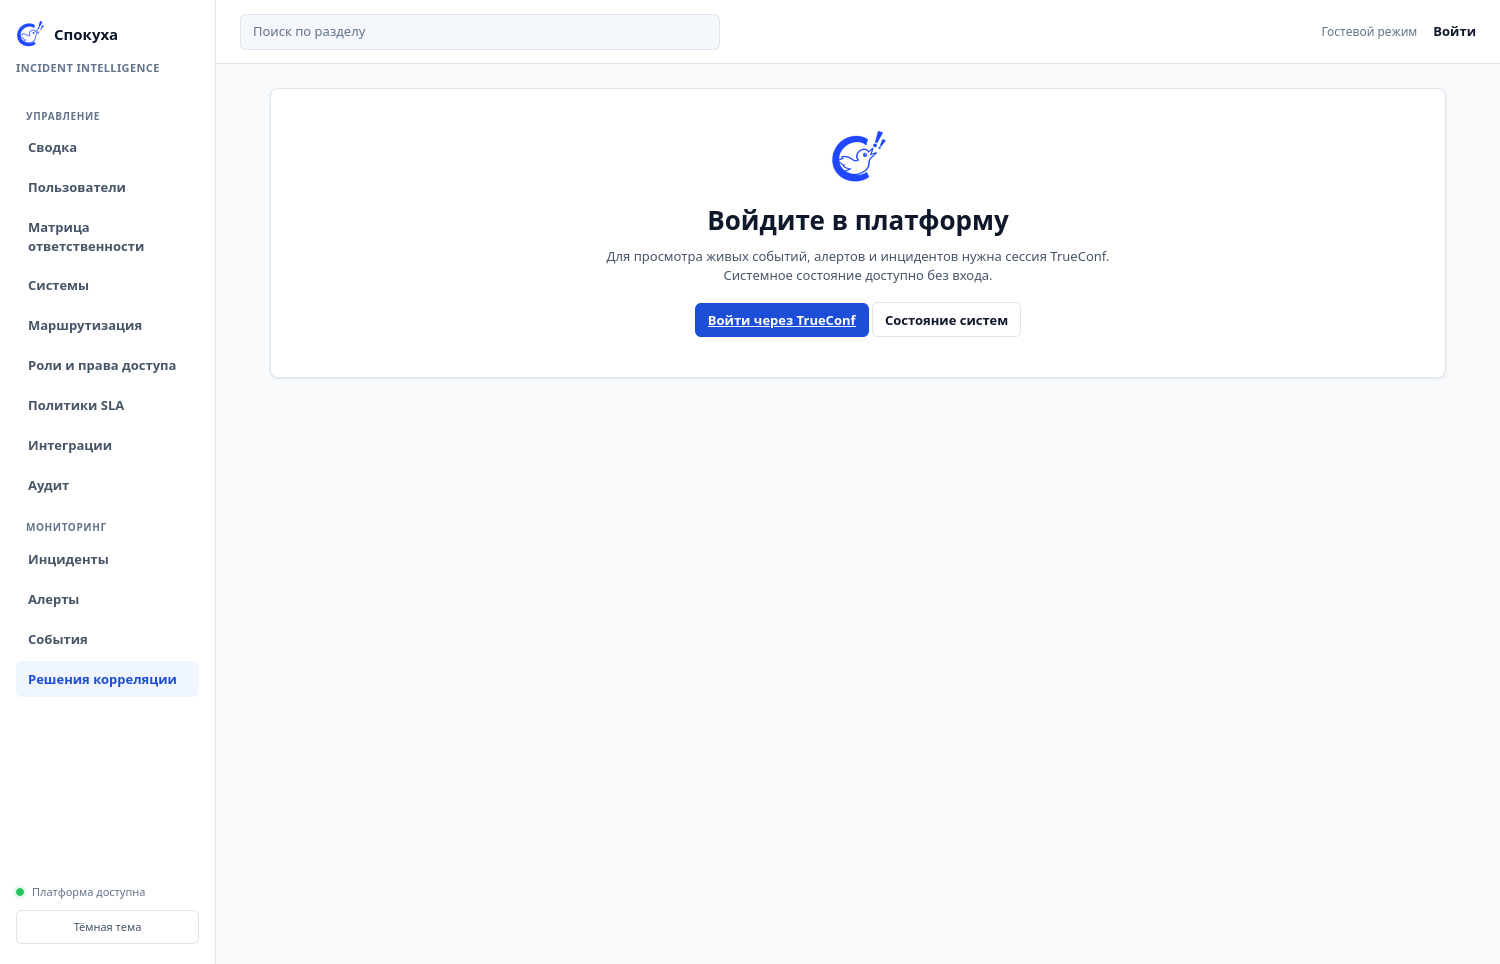
\includegraphics[width=0.85\textwidth]{img/ui-login.png}
    \captionof{figure}{Закрытие разделов мониторинга: вход через TrueConf}
    \label{fig:ui-login}
\end{figure}

Межоригинный вход выполняется по строгому списку
разрешённых адресов возврата, причём токен передаётся во фрагменте URL,
который принципиально не передаётся на сервер.

Объектная авторизация (доступ к конкретному инциденту, активу, подписке) и
второй фактор аутентификации отнесены к целевой архитектуре: объектной модели
инцидентов и подписок на пилоте нет, а второй фактор определяется политикой
корпоративного провайдера входа.

\section{Доступность критического пути}
Ключевое требование~--- сохранение доставки критичного события при отказе
отдельных компонентов. Архитектурно критический путь не зависит от языковой
модели: вызов модели отделён и не создаёт обратного давления, а отказ записи в
хранилище не выходит в поток обработки. Шина сообщений отделяет приём от
обработки и позволяет пережить всплеск без потери событий.

Не реализовано: приоритетные очереди для критичных алертов (сейчас общий
поток), несколько экземпляров критичных сервисов, отдельная очередь
неразбираемых сообщений, технический аварийный обход на существующий механизм
оповещения. На пилоте роль обхода выполняет организационная мера~---
дублирование критичных уведомлений прежним способом.

\section{Данные, секреты и журналы}
\begin{longtable}{|p{3.8cm}|p{6.6cm}|p{4.8cm}|}
\caption{Контроли данных, секретов и журналов}
\label{tab:ibdata} \\
\hline
\rowcolor{edtdark} \hcell{Область} & \hcell{Требуемый контроль} & \hcell{Состояние} \\ \hline
\endfirsthead
\multicolumn{3}{r}{\footnotesize Продолжение таблицы \thetable} \\
\hline
\rowcolor{edtdark} \hcell{Область} & \hcell{Требуемый контроль} & \hcell{Состояние} \\ \hline
\endhead
\endfoot
Секреты & Централизованное хранилище, внедрение в среду выполнения, ротация, запрет хранения в репозитории & \spart Частично: секреты вне репозитория, генерируются случайно, не перезаписываются при развёртывании; централизованного хранилища и ротации нет\\ \hline
Операционные данные & Раздельные сервисные учётные записи БД с минимальными правами & \sdone Не реализовано: одна учётная запись приложения\\ \hline
Аудит & Отдельное хранилище только на дозапись с ограниченным кругом пишущих компонентов & \spart Частично: журнал решений хранится отдельной таблицей с увеличенным сроком (400 дней), но не изолирован как хранилище\\ \hline
Логи & Маскирование токенов, паролей и чувствительных ответов; структурированный формат & \spart Частично: структурированные логи есть, автоматической проверки на секреты нет\\ \hline
Персональные данные & Хранение только технических идентификаторов & \sdone Реализовано: ФИО, телефоны и адреса не хранятся\\ \hline
Сроки хранения & Отдельные сроки для событий, алертов, доставки, аудита и решений & \sdone Реализовано для событий, алертов и решений\\ \hline
\end{longtable}

\section{Сетевая и контейнерная изоляция}
Сетевая модель ограничивает возможность перемещения между компонентами:
интеграции, приложения, данные и ИИ разнесены по разным сетям, хранилище и шина
не публикуют портов наружу, ИИ-контур не имеет исходящего доступа к внешним
сервисам моделей. Представление зон приведено на рисунке~\ref{fig:zones}.

\begin{figure}[H]
    \centering
    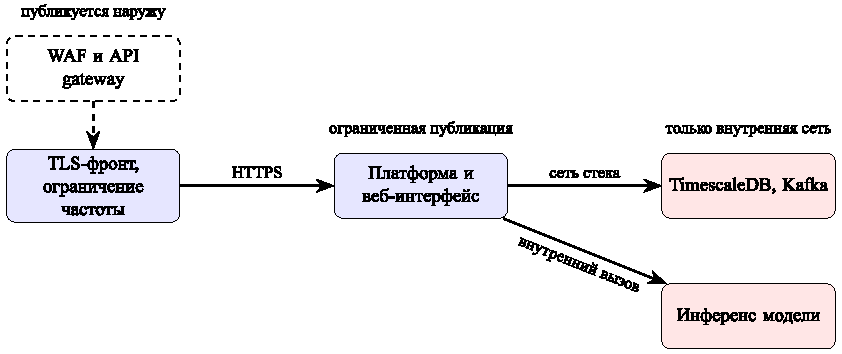
\includegraphics[width=\textwidth]{img/fig-zones.pdf}
    \captionof{figure}{Сетевые зоны и публикуемые точки входа (штриховая рамка~--- целевая архитектура)}
    \label{fig:zones}
\end{figure}

Контейнерная защита реализована частично. Каждый стек имеет собственную сеть и
тома, что ограничивает зону поражения. Требования принципа наименьших
привилегий~--- запуск не от суперпользователя, запрет привилегированного
режима, ограничение возможностей ядра, файловая система только для чтения~---
на пилоте не применены; более того, два вспомогательных стека (агент
мониторинга и контроллер домена) работают в привилегированном режиме, что
приемлемо для стенда и требует пересмотра до промышленной эксплуатации.

\section{Цепочка поставки}
Контроли доверенности артефактов (статический анализ, анализ зависимостей,
сканирование образов и секретов, состав поставки, подпись образов, реестр
моделей с проверкой контрольной суммы) на пилоте не внедрены. Зафиксированы
версии образов в версионируемом файле флагов, что обеспечивает
воспроизводимость, но не доверенность. Домен отнесён к очереди подготовки к
промышленной эксплуатации.

\section{Мониторинг безопасности}
\label{sec:ibmonitor}
Каждый компонент публикует метрики и адрес проверки работоспособности,
включающий состояние подключения к шине и базе. Метрики уведомлений размечены
исходом, что позволяет отслеживать долю немаршрутизируемых алертов.

Особое значение имеет контроль отсутствия ожидаемого потока: молчание источника
неотличимо от исправной работы, если его не контролировать отдельно. Такой
контроль, как и обнаружение всплесков отказов авторизации и массовых изменений
маршрутизации и подписок, отнесён к целевой архитектуре.

\section{Ненейтрализованные угрозы и очерёдность работ}
\label{sec:ibgap}
Здесь угрозы из таблицы~\ref{tab:threats} переводятся в план работ: для каждой
несделанной меры указано фактическое состояние и очередь устранения.
Сводка приведена в таблице~\ref{tab:ibgap}. Столбец очереди
соответствует приоритизации реестра: P0~--- закрывается до промышленной
эксплуатации, P1~--- до вывода в производственный контур.

\begin{longtable}{|p{4.6cm}|p{6.4cm}|p{1.2cm}|p{3.0cm}|}
\caption{Ненейтрализованные угрозы: состояние и очерёдность}
\label{tab:ibgap} \\
\hline
\rowcolor{edtdark} \hcell{Требование реестра} & \hcell{Фактическое состояние} & \hcell{Оч.} & \hcell{Влияние} \\ \hline
\endfirsthead
\multicolumn{4}{r}{\footnotesize Продолжение таблицы \thetable} \\
\hline
\rowcolor{edtdark} \hcell{Требование реестра} & \hcell{Фактическое состояние} & \hcell{Оч.} & \hcell{Влияние} \\ \hline
\endhead
\endfoot
Аутентификация каждого источника событий & Точка приёма webhook доступна без учётных данных; защищена только ограничением частоты и изоляцией сети стенда & \srisk P0 & Подделка событий, ложные аварии \\ \hline
Подтверждение приёма только после надёжного сохранения & Событие публикуется в шину до ответа источнику; отказ записи в проекцию логируется и не поднимается & \srisk P0 & Возможна потеря истории при отказе хранилища \\ \hline
Приоритетные очереди для критичных алертов & Общий поток без приоритизации & \srisk P0 & Задержка критичного при лавине \\ \hline
Отдельная очередь неразбираемых сообщений & Не реализована & \srisk P0 & Повторная обработка некорректных сообщений \\ \hline
Объектная авторизация и второй фактор & Роли есть, объектной модели и второго фактора нет & \srisk P0 & Избыточный доступ администратора \\ \hline
Подписанное подтверждение обработки & Подтверждение реализовано, автор берётся из сессии, а не из тела запроса; криптографической подписи нет & \spart P1 & Ограниченная доказуемость реакции \\ \hline
Централизованное хранилище секретов и ротация & Секреты в приватных файлах вне репозитория, ротации нет & \srisk P0 & Компрометация при доступе к узлу \\ \hline
Технический аварийный обход на прежний механизм & Отсутствует; на пилоте применяется организационное дублирование & \srisk P0 & Простой оповещения при отказе платформы \\ \hline
Контроль отсутствия потока от источника & Не реализован & \srisk P0 & Незамеченное молчание источника \\ \hline
Раздельные учётные записи БД, отдельное хранилище аудита & Одна учётная запись приложения; журнал решений в общей БД & \spart P1 & Смешение операционных и аудиторских данных \\ \hline
Контейнерная защита: без суперпользователя, без привилегий, ограничение возможностей & Не применена; два вспомогательных стека привилегированные & \spart P1 & Расширение зоны поражения \\ \hline
Резервное копирование и регулярные тесты восстановления & Не настроены & \spart P1 & Невосстановимость данных \\ \hline
Несколько экземпляров критичных сервисов & Один узел, единая точка отказа & \spart P1 & Простой при отказе узла \\ \hline
Контроли цепочки поставки & Не внедрены; зафиксированы версии образов & \spart P1 & Уязвимые или подменённые артефакты \\ \hline
Ограничение прав интеграций с \abbr{CMDB} и каталогом & Платформа не обращается к \abbr{CMDB} и каталогу; требование станет применимым при подключении & \sna --- & Неприменимо на пилоте \\ \hline
Контроли поиска по базам знаний & Поиск по базе знаний и векторные представления не используются & \sna --- & Неприменимо к текущей архитектуре \\ \hline
\end{longtable}

Отдельно отмечается, что часть требований реестра выполнена конструктивно и не
требует дополнительных мер: отсутствие персональных данных, отсутствие
полномочий у модели, независимость критичного пути от модели, отсутствие
исходящего доступа ИИ-контура к внешним сервисам.

\section{Доказательство эффективности защитных мер}
Для контролей первой очереди декларативного описания недостаточно: защита
подтверждается функциональным тестом или отрицательным сценарием. Текущее
состояние доказательной базы приведено в таблице~\ref{tab:ibproof}.

\begin{longtable}{|p{8cm}|p{6.4cm}|}
\caption{Проверяемые утверждения о защите}
\label{tab:ibproof} \\
\hline
\rowcolor{edtdark} \hcell{Утверждение} & \hcell{Способ подтверждения} \\ \hline
\endfirsthead
\multicolumn{2}{r}{\footnotesize Продолжение таблицы \thetable} \\
\hline
\rowcolor{edtdark} \hcell{Утверждение} & \hcell{Способ подтверждения} \\ \hline
\endhead
\endfoot
Отключение ИИ не останавливает обработку и доставку критичного алерта & \sdone Автоматический тест: подтверждено\\ \hline
Ответ модели вне объявленного словаря не применяется & \sdone Автоматический тест: подтверждено\\ \hline
Отказ модели, тайм-аут и некорректный JSON приводят к детерминированному тексту & \sdone Автоматический тест: подтверждено\\ \hline
Некорректная нагрузка webhook отклоняется, а не интерпретируется & \sdone Автоматический тест: подтверждено\\ \hline
Два адаптера не могут занять один идентификатор источника & \sdone Автоматический тест: подтверждено\\ \hline
Разделы мониторинга недоступны без аутентификации & \sdone Автоматический тест: подтверждено\\ \hline
Отказ записи в хранилище не прерывает обработку & \sdone Автоматический тест: подтверждено\\ \hline
Неаутентифицированный источник получает отказ & \splan Требует реализации аутентификации источника\\ \hline
Повторная доставка одного события не создаёт новый инцидент & \spart Частично: идентификаторы детерминированы, отдельного теста идемпотентности приёма нет\\ \hline
Критичная очередь сохраняет приоритет при лавине & \splan Требует реализации приоритетных очередей\\ \hline
Секреты отсутствуют в конфигурации и журналах & \splan Требует автоматической проверки\\ \hline
Отказ платформы допускает управляемый переход на прежний механизм & \splan Требует реализации обхода\\ \hline
\end{longtable}


\chapter{Экономика}

\section{Методика и вводные данные}
Финансово-экономическая модель построена по схеме дерева КПЭ: продуктовые
метрики~--- факторы влияния (уровень~4)~--- физические параметры (уровень~3)~---
операционные КПЭ (уровень~2)~--- инвестиционные КПЭ (уровень~1).
Принципиальное отличие настоящего расчёта от оценочного состоит в том, что
нижний уровень дерева не постулируется, а измеряется: значения факторов влияния
сняты прогоном эталонного корпуса через реальный конвейер обработки, а
инварианты, без которых эффект недостижим, зафиксированы автоматическими
тестами.

Все числа модели рассчитываются скриптом \texttt{context/economics.py}:
допущения заданы в нём константами, а таблицы и выводы главы приводят его
результат. Это исключает арифметические расхождения между разделами и
позволяет пересчитать модель под другие ставки одной командой.

Вводные данные, обязательные к использованию, приведены в
таблице~\ref{tab:econ-given}; собственные допущения выделены отдельно
(таблица~\ref{tab:econ-input}) и снабжены обоснованием.

\begin{table}[H]
\centering
\caption{Обязательные вводные данные}
\label{tab:econ-given}
\resizebox{\textwidth}{!}{%
\begin{tabular}{|p{7cm}|p{3.5cm}|p{5cm}|}
\hline
\rowcolor{edtdark} \hcell{Параметр} & \hcell{Значение} & \hcell{Применение} \\ \hline
Стоимость \abbr{FTE} (с учётом взносов и накладных расходов) & 2\,000 руб./ч & Расчёт эффектов \\ \hline
Стоимость часа работы проектной команды & 3\,500 руб./ч & Расчёт расходной части \\ \hline
Стоимость простоя установки НПЗ & 150 млн руб./сут. (6,25 млн руб./ч) & Расчёт эффекта от сокращения простоя \\ \hline
\end{tabular}%
}
\end{table}

\section{Источники измерения}
\textbf{Симуляция.} Эталонный корпус (1053~алерта, 8~инцидентов, 2~часа
модельного времени, фиксированный seed) прогоняется через реальный конвейер.
Эталонная разметка в конвейер не попадает: в метки алерта передаются только
сервис, среда, площадка, объект и команда-владелец, а признаки
«значимый/шумовой» и идентификатор инцидента доступны только измерителю.
Иначе корреляция сгруппировала бы алерты по идентификатору инцидента и показала
бы идеальный результат по неверной причине.

\textbf{Тесты.} Автоматические тесты фиксируют инварианты, на которых держится
модель эффекта: недоступность языковой модели не прерывает доставку, отказ
записи в хранилище не выходит в поток обработки, уверенность всегда лежит в
отрезке [0;\,1], ответ модели вне словаря отбрасывается. Текущее состояние~---
145~пройденных тестов платформы, 1~пропущенный (требует развёрнутой модели),
4~отмеченных как известные ограничения; отдельно покрыты диспетчер доставки и
генератор событий. Расчёт эффекта предполагает, что критичное уведомление
доходит и при отказе ИИ~--- это утверждение проверяется тестом, а не
декларируется.

\section{Продуктовые метрики (база и цель)}
Продуктовые метрики и факторы влияния уровня~4~--- это одни и те же величины,
снятые с симуляции (таблица~\ref{tab:kpi}). Целевые значения задаются
относительно измеренной базовой линии и снимаются тем же способом:
на корпусе~--- прогоном измерителя, в эксплуатации~--- метриками платформы.

\begin{table}[H]
\centering
\caption{Продуктовые метрики: базовое и целевое значения}
\label{tab:kpi}
\resizebox{\textwidth}{!}{%
\begin{tabular}{|p{5cm}|c|c|c|p{4.2cm}|}
\hline
\rowcolor{edtdark} \hcell{Метрика} & \hcell{База} & \hcell{Достигнуто} & \hcell{Цель} & \hcell{Способ измерения} \\ \hline
Уведомлений за 2 ч корпуса, шт. & 1053 & 44 & $\le 50$ & Измеритель на корпусе \\ \hline
Уведомлений в час, шт. & 527 & 22 & $\le 25$ & Метрики платформы \\ \hline
Уведомлений на один инцидент, шт. & 132 & 5,5 & $\le 6$ & Измеритель; метрики решений \\ \hline
Шумовых уведомлений, шт. & 508 & 17 & $\le 10$ & Измеритель по эталону \\ \hline
Уведомлений не тому адресату, шт. & 329 & 13 & $\le 5$ & Измеритель; обратная связь дежурных \\ \hline
Доля полезных уведомлений & 20,5\,\% & 31,8\,\% & $\ge 60\,\%$ & Измеритель по владельцу сервиса \\ \hline
Полнота обнаружения инцидентов & 8/8 & 8/8 & 8/8 & Измеритель; сверка с журналом аварий \\ \hline
Время до первого уведомления & --- & --- & $\le 15$ с & Метрики платформы \\ \hline
Доля немаршрутизируемых алертов & --- & --- & $\le 5\,\%$ & Метрика маршрутизации \\ \hline
Доставка при недоступности ИИ & --- & 100\,\% & 100\,\% & Тесты отказа модели \\ \hline
\end{tabular}%
}
\end{table}

Полнота вынесена в таблицу как контрольная метрика: снижение числа уведомлений
при потере хотя бы одного инцидента из восьми было бы неприемлемо для
промышленной эксплуатации. Именно поэтому правило эскалации, восстановившее
полноту до 8/8 ценой восьми дополнительных уведомлений и 0,8~процентного пункта
снижения шума, является правильным разменом, а не ухудшением результата.
Достижение целевой доли полезных уведомлений (60\,\%) требует учёта
первопричины при маршрутизации: измерение показало, что 13 из 44~уведомлений
уходят дежурному сигнализирующего, а не сломавшегося сервиса. Экономическая
цель и техническая задача следующего этапа здесь~--- одно и то же утверждение,
проверяемое на том же корпусе.

\section{Собственные допущения}
\begin{table}[H]
\centering
\caption{Собственные допущения и их обоснование}
\label{tab:econ-input}
\resizebox{\textwidth}{!}{%
\begin{tabular}{|p{5cm}|p{2.5cm}|p{8cm}|}
\hline
\rowcolor{edtdark} \hcell{Параметр} & \hcell{Значение} & \hcell{Обоснование} \\ \hline
Поток алертов пилотного периметра & 12\,636 шт./сут. & Экстраполяция измеренного корпуса на сутки ($\times$\,12) \\ \hline
Среднее время реакции на уведомление & 2 мин & Оценка времени открыть, прочитать и квалифицировать оповещение \\ \hline
Дежурные смены & 2 по 8 ч & Типовая организация дежурства на пилотном периметре \\ \hline
Доля времени дежурного на разбор оповещений & 30\,\% & Ограничивает эффект сверху фактическим фондом времени \\ \hline
Доля высвобождаемого времени & 70\,\% & Часть разбора остаётся при любом снижении шума \\ \hline
Значимых инцидентов с простоем в год & 6 & Пилотный периметр; уточняется по журналу аварий \\ \hline
Сокращение времени обнаружения и адресации на инцидент & 15 мин & Следствие снижения со 132 до 5,5 уведомлений на инцидент и адресной доставки \\ \hline
Состав проектной команды & 6 человек & Архитектор, три разработчика, специалист по ИБ, аналитик \\ \hline
Трудоёмкость разработки и внедрения пилота & 1\,920 ч & 6 человек $\times$ 8 недель $\times$ 40 ч \\ \hline
Трудоёмкость сопровождения & 30 ч/мес & Поддержка адаптеров, правил и конфигурации \\ \hline
Инфраструктура: три узла (приложения, данные и шина, ИИ с \abbr{GPU}) & 0,76 млн руб./год & Конфигурации из таблицы~\ref{tab:sizing}; расчёт стоимости~--- таблица~\ref{tab:infracost} \\ \hline
Ставка дисконтирования & 20\,\% & Типовая для ИТ-проектов внутренней автоматизации \\ \hline
Горизонт расчёта & 3 года & Соответствует сроку жизни пилотного решения до пересмотра \\ \hline
\end{tabular}%
}
\end{table}

\section{Дерево КПЭ}
Переход от измеренных метрик к деньгам выполняется в два шага: факторы влияния
пересчитываются в физические параметры (человеко-часы, часы простоя), а те~---
в операционные КПЭ по обязательным ставкам (рисунок~\ref{fig:kpi-tree}).

\begin{landscape}
\begin{figure}[H]
    \centering
    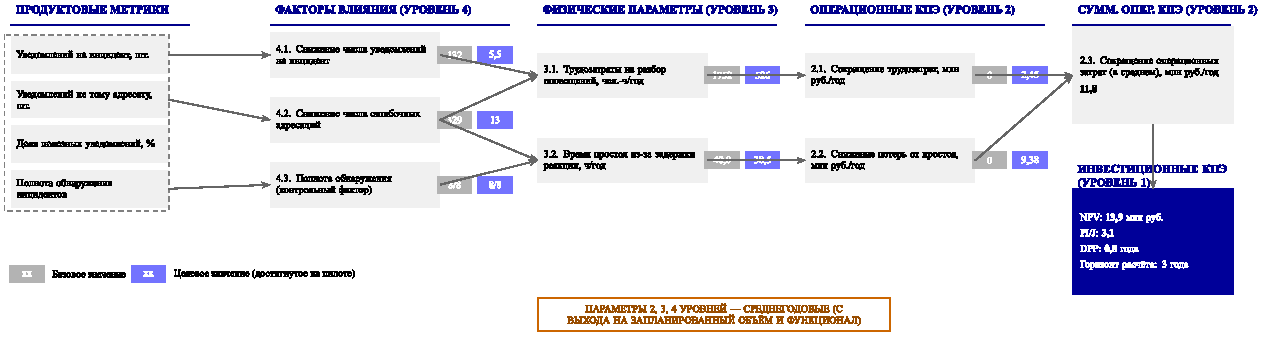
\includegraphics[width=\linewidth]{img/fig-kpi-tree.pdf}
    \captionof{figure}{Дерево КПЭ: от продуктовых метрик к инвестиционным показателям}
    \label{fig:kpi-tree}
\end{figure}
\end{landscape}

\textbf{Физический параметр 3.1~--- сокращение трудозатрат на разбор
оповещений.} Прямое умножение сокращённого потока (12\,204 уведомления в сутки)
на время реакции даёт 407~человеко-часов в сутки, что заведомо превышает фонд
рабочего времени дежурных. Такой расчёт был бы неверен: эти часы сегодня не
тратятся, поток игнорируется~--- и именно через это теряются аварии. Поэтому
эффект ограничивается фактическим фондом: две смены по 8~часов дают
16~человеко-часов в сутки, из которых 30\,\% приходится на разбор
оповещений~--- 4,8~человеко-часа. Высвобождается 70\,\% этой величины:
$4{,}8 \times 0{,}7 = 3{,}36$~человеко-часа в сутки, или
$3{,}36 \times 365 \approx 1\,226$~человеко-часов в год.

\textbf{Физический параметр 3.2~--- сокращение времени простоя.} Снижение числа
уведомлений на инцидент со 132 до 5,5 и сокращение ошибочной адресации с 329 до
13~случаев означают, что авария перестаёт тонуть в потоке и попадает
ответственному дежурному сразу. Принимается сокращение времени обнаружения и
адресации на 15~минут на инцидент при 6~значимых инцидентах в год:
$6 \times 0{,}25 = 1{,}5$~часа простоя в год.

\textbf{Операционные КПЭ.} По обязательным ставкам:
\begin{itemize}
    \item 2.1: $1\,226 \times 2\,000 = 2{,}45$ млн руб./год;
    \item 2.2: $1{,}5 \times 6{,}25 = 9{,}38$ млн руб./год.
\end{itemize}
Суммарный операционный эффект~--- \textbf{11,8 млн руб./год}.

\section{Затраты}
Расходная часть рассчитана по ставке 3\,500 руб./ч
(таблица~\ref{tab:econ-cost}). Лицензионные отчисления за внешние сервисы
отсутствуют: все компоненты, включая инференс языковой модели, размещены в
корпоративном контуре.

\begin{table}[H]
\centering
\caption{Структура затрат}
\label{tab:econ-cost}
\resizebox{\textwidth}{!}{%
\begin{tabular}{|p{6cm}|p{3cm}|p{2.8cm}|p{4cm}|}
\hline
\rowcolor{edtdark} \hcell{Статья} & \hcell{Расчёт} & \hcell{Сумма} & \hcell{Характер} \\ \hline
Разработка и внедрение пилота (6 человек, 8 недель) & $1\,920 \times 3\,500$ & 6,7 млн руб. & Разовые \\ \hline
Сопровождение и развитие & $360 \times 3\,500$ & 1,3 млн руб./год & Периодические \\ \hline
Инфраструктура: три узла (см. таблицу~\ref{tab:infracost}) & $63\,000 \times 12$ & 0,76 млн руб./год & Периодические \\ \hline
Лицензии внешних сервисов & --- & 0 & --- \\ \hline
\multicolumn{2}{|l|}{\textbf{Итого разовые}} & \textbf{6,7 млн руб.} & \\ \hline
\multicolumn{2}{|l|}{\textbf{Итого периодические}} & \textbf{2,0 млн руб./год} & \\ \hline
\end{tabular}%
}
\end{table}

\subsection*{Стоимость инфраструктуры}
Стоимость посчитана для аренды вычислительных ресурсов; альтернатива~---
приобретение сервера с \abbr{GPU} в собственность~--- переносит основную часть суммы
из периодических затрат в разовые и рассматривается как вариант при переходе к
промышленной эксплуатации (таблица~\ref{tab:infracost}).

\begin{table}[H]
\centering
\caption{Стоимость инфраструктуры при аренде}
\label{tab:infracost}
\begin{tabular}{|p{5.4cm}|p{4.6cm}|p{3.4cm}|}
\hline
\rowcolor{edtdark} \hcell{Узел} & \hcell{Конфигурация} & \hcell{Стоимость, руб./мес.} \\ \hline
Приложения & 4 vCPU, 8 ГБ, 50 ГБ & 6\,000 \\ \hline
Данные и шина & 8 vCPU, 16 ГБ, 200 ГБ SSD & 12\,000 \\ \hline
ИИ (\abbr{GPU})~\cite{vllm} & 8 vCPU, 32 ГБ, \abbr{GPU} 16 ГБ & 45\,000 \\ \hline
\textbf{Итого} & & \textbf{63\,000} \\ \hline
\end{tabular}
\end{table}

Цены являются допущением и подлежат уточнению по действующим договорам;
структура расчёта от них не зависит. Доля ИИ-узла составляет 71\,\% стоимости
инфраструктуры~--- это прямое следствие того, что модель постоянно удерживает
видеопамять. При отключённых ИИ-функциях (режим off) годовая стоимость
инфраструктуры снижается с 0,76 до 0,22 млн руб.

\subsection*{Альтернативный сценарий: приобретение оборудования}
Ориентировочная оценка капитальных затрат при переходе от аренды к
собственному оборудованию приведена в таблице~\ref{tab:capex}. Цены заданы
по порядку величины исходя из типовой конфигурации серверов корпоративного
класса и подлежат уточнению по коммерческим предложениям поставщиков;
основной источник неопределённости~--- стоимость \abbr{GPU}-карты с
16~ГБ видеопамяти.

\begin{table}[H]
\centering
\caption{Оценка капитальных затрат на оборудование}
\label{tab:capex}
\begin{tabular}{|p{5.4cm}|p{4.6cm}|p{3.4cm}|}
\hline
\rowcolor{edtdark} \hcell{Узел} & \hcell{Конфигурация} & \hcell{Стоимость, млн руб.} \\ \hline
Приложения & 4 vCPU, 8 ГБ, 50 ГБ & 0,25 \\ \hline
Данные и шина & 8 vCPU, 16 ГБ, 200 ГБ SSD & 0,45 \\ \hline
ИИ (\abbr{GPU}) & 8 vCPU, 32 ГБ, \abbr{GPU} 16 ГБ & 1,66 \\ \hline
\textbf{Итого} & & \textbf{2,36} \\ \hline
\end{tabular}
\end{table}

Приобретение не обнуляет периодические расходы на инфраструктуру: остаются
размещение в дата-центре, электроэнергия и обслуживание. Эта часть оценена
в 15\,\% стоимости оборудования в год~--- 0,35~млн~руб./год вместо
0,76~млн~руб./год при аренде. Итоговые периодические затраты снижаются
с 2,0 до 1,65~млн~руб./год, а разовые инвестиции возрастают с 6,7 до
9,06~млн~руб. (таблица~\ref{tab:capex-npv}); методика дисконтирования~---
та же, что и в таблице~\ref{tab:econ-npv}.

\begin{table}[H]
\centering
\caption{Сравнение сценариев аренды и приобретения оборудования}
\label{tab:capex-npv}
\begin{tabular}{|l|c|c|}
\hline
\rowcolor{edtdark} \hcell{Показатель} & \hcell{Аренда} & \hcell{Приобретение} \\ \hline
Разовые инвестиции, млн руб. & 6,7 & 9,06 \\ \hline
Периодические затраты, млн руб./год & 2,0 & 1,65 \\ \hline
\textbf{NPV} на горизонте 3 года, млн руб. & 13,9 & 12,3 \\ \hline
\textbf{DPP}, лет & 0,8 & 1,1 \\ \hline
\end{tabular}
\end{table}

Оба сценария окупаются в пределах горизонта расчёта. Аренда даёт более
быстрый \abbr{DPP} за счёт меньших разовых вложений; приобретение~---
немного ниже итоговый \abbr{NPV} из-за более высокой стартовой инвестиции
при том же операционном эффекте. Разница \abbr{NPV} (1,6~млн~руб.) меньше
точности допущений о ценах на оборудование, поэтому выбор между сценариями
определяется доступностью капитальных статей бюджета на этапе пилота, а не
экономической целесообразностью.

\section{Инвестиционные КПЭ}
Чистый денежный поток года: $11{,}8 - 2{,}0 = 9{,}8$~млн~руб. Дисконтирование
по ставке 20\,\% на горизонте 3~года приведено в
таблице~\ref{tab:econ-npv}.

\begin{table}[H]
\centering
\caption{Финансово-экономическая модель, млн руб.}
\label{tab:econ-npv}
\begin{tabular}{|l|c|c|c|c|}
\hline
\rowcolor{edtdark} \hcell{Показатель} & \hcell{Год 0} & \hcell{Год 1} & \hcell{Год 2} & \hcell{Год 3} \\ \hline
Эффект                       & ---   & 11,8 & 11,8 & 11,8 \\ \hline
Операционные затраты         & ---   & 2,0  & 2,0  & 2,0  \\ \hline
Инвестиции                   & 6,7   & ---  & ---  & ---  \\ \hline
Чистый поток                 & $-6{,}7$ & 9,8 & 9,8 & 9,8 \\ \hline
Коэффициент дисконтирования  & 1,00  & 0,83 & 0,69 & 0,58 \\ \hline
Дисконтированный поток       & $-6{,}7$ & 8,2 & 6,8 & 5,7 \\ \hline
Накопленный дисконт. поток   & $-6{,}7$ & 1,5 & 8,3 & 13,9 \\ \hline
\end{tabular}
\end{table}

\begin{itemize}
    \item \textbf{NPV} = 13,9 млн руб. на горизонте 3~года;
    \item \textbf{PV} = 20,7 млн руб., \textbf{PVI} = 6,7 млн руб.,
          \textbf{PI} = 3,1;
    \item \textbf{DPP} $\approx$ 0,8 года (около 10~месяцев).
\end{itemize}

\section{Чувствительность и риски модели}
Модель определяется главным образом эффектом от простоя: при стоимости
6,25~млн~руб. за час достаточно предотвратить 1,4~часа простоя в год, чтобы
покрыть все затраты первого года (8,7~млн~руб.). Отсюда следуют два вывода.

Во-первых, точность оценки числа значимых инцидентов и сокращения времени
реакции важнее точности оценки трудозатрат: даже полное обнуление эффекта 2.1
оставляет проект окупаемым (\abbr{NPV} $\approx$ 8,8 млн руб.), тогда как ошибка в
1~час простоя меняет годовой эффект на 6,25 млн руб.

Во-вторых, главный экономический риск~--- не переоценка эффекта, а потеря
инцидента: один пропущенный бизнес-критичный инцидент при указанной стоимости
простоя способен обнулить годовой эффект целиком. На эталонном корпусе полнота
доведена до 8/8, однако это измерение на синтетическом потоке, а не на реальном
трафике, поэтому дублирование критичных уведомлений существующим способом
сохраняется на время пилота, а полнота остаётся в дереве КПЭ контрольным
фактором, а не второстепенной метрикой качества.


% \printnomenclature % Автоматический список сокращений

\frontmatter % выключает нумерацию ВСЕГО; здесь начинаются ненумерованные главы


\backmatter %% Здесь заканчивается нумерованная часть
\Conclusion
В ходе работы спроектирована и реализована веб-платформа управления
оповещениями для пилотного периметра, отвечающая обоим ограничениям кейса:
она не обрабатывает реальные персональные данные и не зависит от домена
Active Directory. Роль AD в контуре идентификации выполняет TrueConf: он
служит одновременно каналом доставки и провайдером аутентификации.

Получены следующие результаты:
\begin{itemize}
    \item построена архитектура с детерминированным ядром обработки и
          необязательным ИИ-контуром, трассированная на требования заказчика
          (приложение~\ref{app:traceability});
    \item реализован приём разноформатных событий через сменные адаптеры
          (Alertmanager, Zabbix, генератор синтетических событий) с приведением
          к единой открытой схеме;
    \item реализована корреляция алертов конечным автоматом с решениями
          дедупликации, подавления и маршрутизации;
    \item реализованы дашборд и личный кабинет с разделением ролей и
          настраиваемой ролевой моделью;
    \item реализована сквозная доставка уведомлений в TrueConf с фиксацией
          статуса и детерминированным резервным путём;
    \item реализованы два ИИ-сценария (обогащение алерта и формулировка
          уведомления) с локальным инференсом, объяснимостью и полным
          fallback-поведением;
    \item построен воспроизводимый корпус и измерено качество обработки:
          снижение числа уведомлений на 95,8\,\% при полной обнаруживаемости
          инцидентов~--- 8~из~8 (таблица~\ref{tab:scoring});
    \item подготовлено экономическое обоснование с явно выделенными
          допущениями.
\end{itemize}

Выявленные ограничения~--- слияние одновременных инцидентов на общем сервисе
и адресация по владельцу сигнализирующего, а не сломавшегося сервиса~---
измерены количественно и определяют содержание следующего этапа: учёт
первопричины и данных сервисного каталога при корреляции и маршрутизации,
а также реализация инцидента как самостоятельной сущности с карточкой,
подтверждением обработки и каналом обратной связи по решениям ИИ.

% цитируем ВСЁ
\nocite{*}
\include{81-biblio}

\appendix   % Тут идут приложения

\chapter{Матрица трассировки требований на архитектурные решения}
\label{app:traceability}
Матрица связывает требования заказчика с архитектурными решениями и критериями
их проверки. Идентификаторы требований сохранены в форме, предоставленной
заказчиком. Решения описываются как компоненты и их обязанности: конкретные
продукты не фиксируются там, где выбор не сделан.

\begin{longtable}{|p{1.1cm}|p{5.4cm}|p{3.4cm}|p{5.4cm}|}
\caption{Матрица трассировки требований на архитектурные решения}
\label{tab:traceability} \\
\hline
\rowcolor{edtdark} \hcell{ID} & \hcell{Архитектурное решение} & \hcell{Требования-основания} & \hcell{Критерий приёмки} \\ \hline
\endfirsthead
\multicolumn{4}{r}{\footnotesize Продолжение таблицы \thetable} \\
\hline
\rowcolor{edtdark} \hcell{ID} & \hcell{Архитектурное решение} & \hcell{Требования-основания} & \hcell{Критерий приёмки} \\ \hline
\endhead
\endfoot
АР-01 & Ввести единый контур приёма событий: \abbr{API} gateway/\abbr{WAF}, push webhook/HTTP и индивидуальные конфигурируемые адаптеры для каждой системы мониторинга. Адаптеры приводят события к единой внутренней схеме. & БТ-1; ФТ1.1, ФТ1.2, ФТ1.4; НФТ1.4; НФТ4.1, НФТ4.11, НФТ4.13 & Новый источник подключается маппингом полей без изменения кода; событие принимается по защищённому каналу и нормализуется; отказ адаптера не приводит к потере накопленных событий. \\ \hline
АР-02 & Использовать устойчивую асинхронную шину событий с очередями, consumer groups, приоритизацией, backpressure и отдельной очередью ошибок (\abbr{DLQ}). & БТ-1; НФТ1.4; НФТ4.5, НФТ4.9, НФТ4.12; ФТ6.3; НФТ7.3 & При недоступности потребителя события сохраняются и обрабатываются после восстановления; критичные алерты имеют приоритет; RPO = 0 и RTO приёма не более 3 минут. \\ \hline
АР-03 & Реализовать детерминированное ядро обработки: настраиваемые правила критичности, типизации, дедупликации и корреляции. Это гарантированный путь обработки, независимый от \abbr{LLM}. & БТ-2; ПТ2.1; ФТ2.1, ФТ2.2, ФТ2.3; БТ-6; ФТ6.2, ФТ6.3; НФТ6.1; БТ-7; ПТ7.2, ПТ7.3; НФТ7.2 & Правила меняются без переработки истории; при отключённом AI события классифицируются, коррелируются, маршрутизируются и доставляются. \\ \hline
АР-04 & Хранить классификации, правила, пороги уверенности, режимы автоматизации и fallback-политику как конфигурацию с версионированием, а не как жёстко заданный код. & ПТ2.1; НФТ2.3; ФТ6.1; ПТ7.1, ПТ7.2; ФТ7.6; НФТ7.1 & Новая категория добавляется без пересчёта истории; для каждой AI-функции задаются режим, confidence threshold и fallback; версия политики видна в аудите. \\ \hline
АР-05 & Предоставить централизованный web frontend: дашборд администратора и личный кабинет пользователя с текущими авариями, поиском, историей, аудитом, подписками и политиками. & ПТ2.2; ПТ3.1; НФТ2.1; НФТ3.1; ФТ7.7 & Новое событие видно на панели не позднее 15 секунд; изменение подписки в UI получает отклик не позднее 3 секунд; пользователь может подтвердить, отклонить или переопределить AI-решение. \\ \hline
АР-06 & Выделить компонент маршрутизации и уведомлений: подписки по источнику/типу/критичности/активу, шаблоны уведомлений, обязательная интеграция с TrueConf, опциональные каналы, статус доставки и fallback. & БТ-3; ФТ3.1, ФТ3.2, ФТ3.4, ФТ3.5, ФТ3.7; НФТ3.2, НФТ3.3, НФТ3.4; НФТ4.14 & Изменённая подписка применяется к новым событиям не позднее 5 секунд; при недоступности основного канала fallback срабатывает не позднее 1 минуты; доставка каждого уведомления имеет зафиксированный статус. \\ \hline
АР-07 & Использовать OAuth 2 через TrueConf как основной путь аутентификации; поддержать локальные учётные записи. AD использовать только как номинальный справочник для статуса/атрибутов пользователя, без зависимости от реального AD на пилоте. & БТ-4; ФТ4.1, ФТ4.2, ФТ4.3; НФТ4.3, НФТ4.4 & Пользователь аутентифицируется через TrueConf или локальную учётную запись; права назначаются ролями и группами; подписки деактивируются при сигнале о кадровом изменении; в БД нет ФИО, телефонов и иных \abbr{ПДн}. \\ \hline
АР-08 & Хранить в TimescaleDB (PostgreSQL-совместимая БД) события, алерты и статусы доставки в hypertables с настраиваемыми retention и сжатием; хранить состояние инцидентов, подписки, политики, аудит и только технические, псевдонимизированные идентификаторы пользователей как реляционные записи. & ФТ1.6; НФТ4.2, НФТ4.4; НФТ7.1 & История за заданный временной диапазон доступна в пределах retention; hypertables сжимаются по политике; журнал действий хранится не менее года; журнал AI-решений содержит модель, версию, confidence, входные признаки и результат. \\ \hline
АР-09 & Использовать \abbr{CMDB}/сервисный каталог как источник контекста: объекты, сервисы, владельцы, команды, on-call и зоны ответственности. Кэшировать горячий контекст, чтобы не сделать \abbr{CMDB} bottleneck. & ФТ3.1; ФТ7.3, ФТ7.4; НФТ4.12 & Маршрут определяется по активу и владельцу; при низкой уверенности алерт направляется в triage-очередь; недоступность или медленность \abbr{CMDB} не блокирует приём критичных алертов. \\ \hline
АР-10 & Реализовать отдельный необязательный AI-контур через асинхронный worker и контракт сообщений. Поддержать функции: семантическая дедупликация, фильтрация шума/карантин, приоритизация, маршрутизация, саммаризация, декомпозиция и объяснение решений. & БТ-2; ФТ2.2, ФТ2.3, ФТ2.4; БТ-7; ФТ7.1-ФТ7.7; НФТ7.1-НФТ7.4 & AI-решение содержит explanation, confidence, признаки, альтернативы и версию модели; critical/high не скрываются, не подавляются и не понижаются автоматически; при низкой уверенности применяется triage/fallback. \\ \hline
АР-11 & Размещать LLM-инференс и дообучение только в корпоративном контуре. Выделить внутренний \abbr{LLM} gateway/балансировщик и управляемый пул inference; исключить внешние облачные \abbr{API} для модели. & НФТ2.2; НФТ7.4 & Сетевые политики исключают исходящий доступ AI-контура к внешним \abbr{LLM} \abbr{API}; инвентаризация показывает, что модели, inference и обучение находятся в контуре компании. \\ \hline
АР-12 & Не делать AI/\abbr{LLM} синхронной точкой отказа основного потока. При сбое AI применять детерминированные правила и зафиксированное fallback-поведение; использовать feature flags и режимы off/shadow/suggest/assisted auto/full auto. & БТ-6; ФТ6.1-ФТ6.3; НФТ6.1; ПТ7.1-ПТ7.3; НФТ7.2, НФТ7.3 & Отключение AI worker или inference не задерживает приём, регистрацию и доставку critical-алерта; режим AI переключается без развёртывания ядра. \\ \hline
АР-13 & Построить наблюдаемость и аудит как сквозную функцию: структурированные логи, метрики, трассировка, Kafka lag, SLO, аудит пользователей, изменений БД, решений AI и статусов доставки. Исключать секреты и чувствительные данные из логов. & НФТ4.2, НФТ4.8, НФТ4.10; НФТ7.1; НФТ3.4; НФТ2.1 & Можно отследить путь события от приёма до доставки; можно доказать, кто изменил правило/подписку; автоматическая проверка не обнаруживает секретов или чувствительных данных в логах. \\ \hline
АР-14 & Применить defense in depth: \abbr{TLS} 1.2+, сегментация сети, закрытые БД/очереди, минимальные привилегии, индивидуальные service accounts, секреты в vault, резервное копирование и регулярные тесты восстановления. & НФТ4.1, НФТ4.5-НФТ4.10 & Внешние интеграции используют \abbr{TLS} 1.2+; доступ к БД и очередям ограничен сетевыми правилами и сервисными учётными записями; восстановление из backup регулярно проверяется. \\ \hline
АР-15 & Защищать входной и исходящий трафик: \abbr{WAF}/\abbr{API} gateway, rate limiting для \abbr{API}/аутентификации, квоты на уведомления, защита от alert storm и отдельная политика critical-приоритета. & НФТ4.11-НФТ4.14; НФТ1.4 & Аномальный HTTP-трафик ограничивается на периметре; лавина событий не обрушает обработку; квоты предотвращают массовую рассылку, не блокируя допустимые critical-эскалации. \\ \hline
АР-16 & Вести пилот через поэтапное подключение источников, feature flags, критерии успеха, документированный rollback и временное дублирование критичных уведомлений. & БТ-5; ПТ5.1-ПТ5.3; НФТ5.1; ФТ6.1 & Каждый этап имеет список источников, метрики успеха, владельца и rollback-план; критичные уведомления можно временно дублировать; откат укладывается в согласованное значение X минут. \\ \hline
АР-17 & Включить симулятор событий как равноправный тестовый источник, использующий те же схемы, адаптеры и поток обработки, что и реальные системы мониторинга. & БЦ; БТ-1; ФТ1.1, ФТ1.4; НФТ1.4; БТ-5; ПТ5.1, ПТ5.2 & Без доступа к инфраструктуре компании симулятор создаёт сценарии normal/critical/storm/failure; они проходят полный путь до dashboard и уведомления и используются для проверки rollout/rollback. \\ \hline
\end{longtable}

\chapter{Детальная схема архитектуры}
\label{app:architecture}
Схема объединяет все представления главы~1 и приводится как справочный
материал: она перегружена для чтения по ходу текста, но полезна как единая
карта компонентов и связей.

\begin{figure}[H]
    \centering
    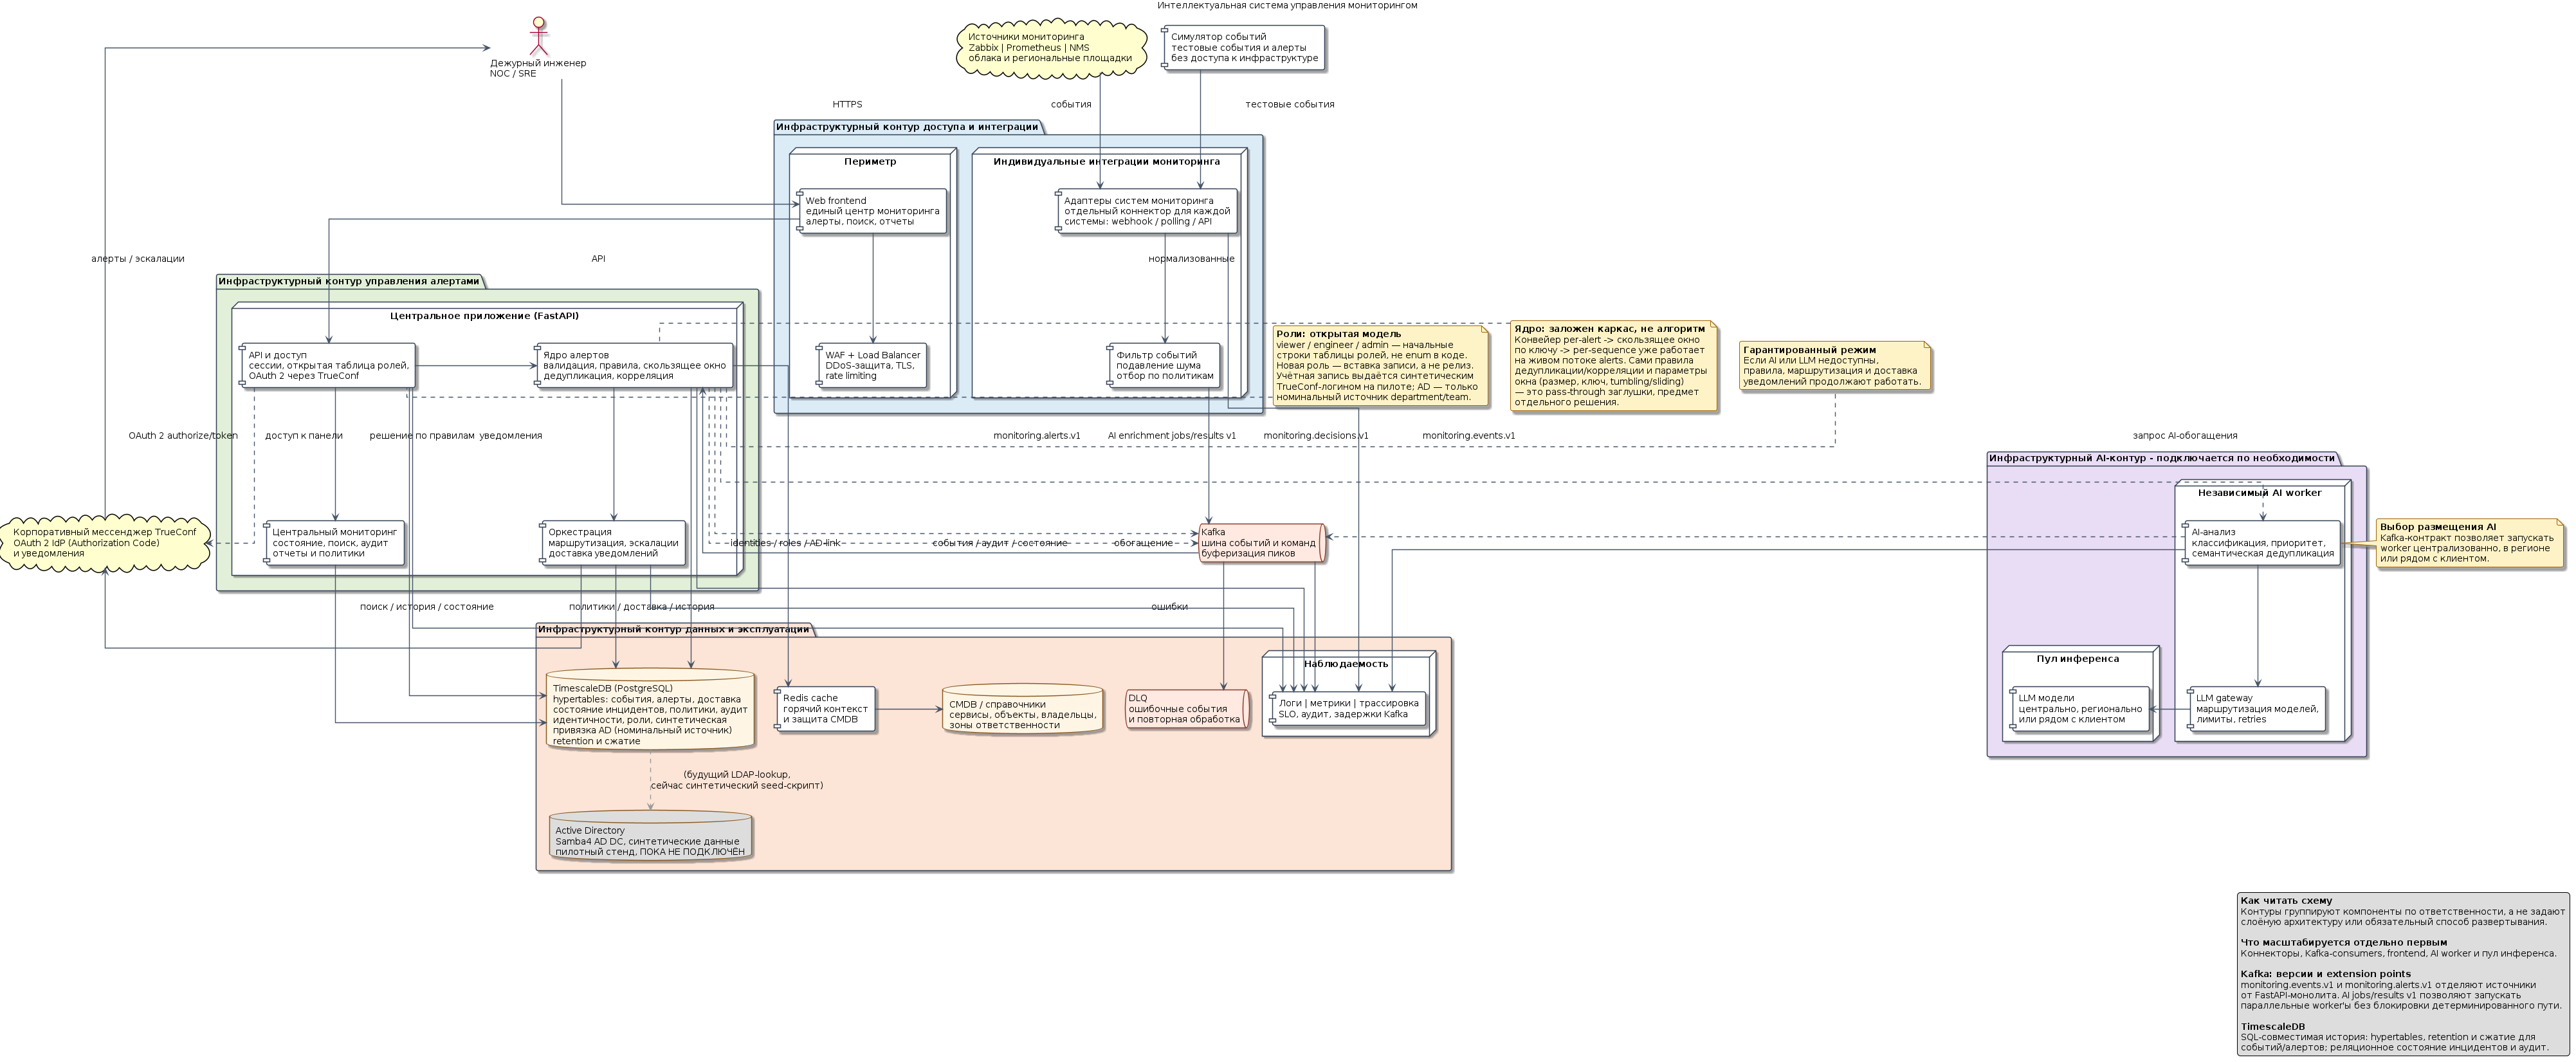
\includegraphics[width=\textwidth]{img/architecture.png}
    \captionof{figure}{Детальная схема архитектуры решения}
    \label{fig:architecture}
\end{figure}

\chapter{Схема данных}
\label{app:erd}

\begin{figure}[H]
    \centering
    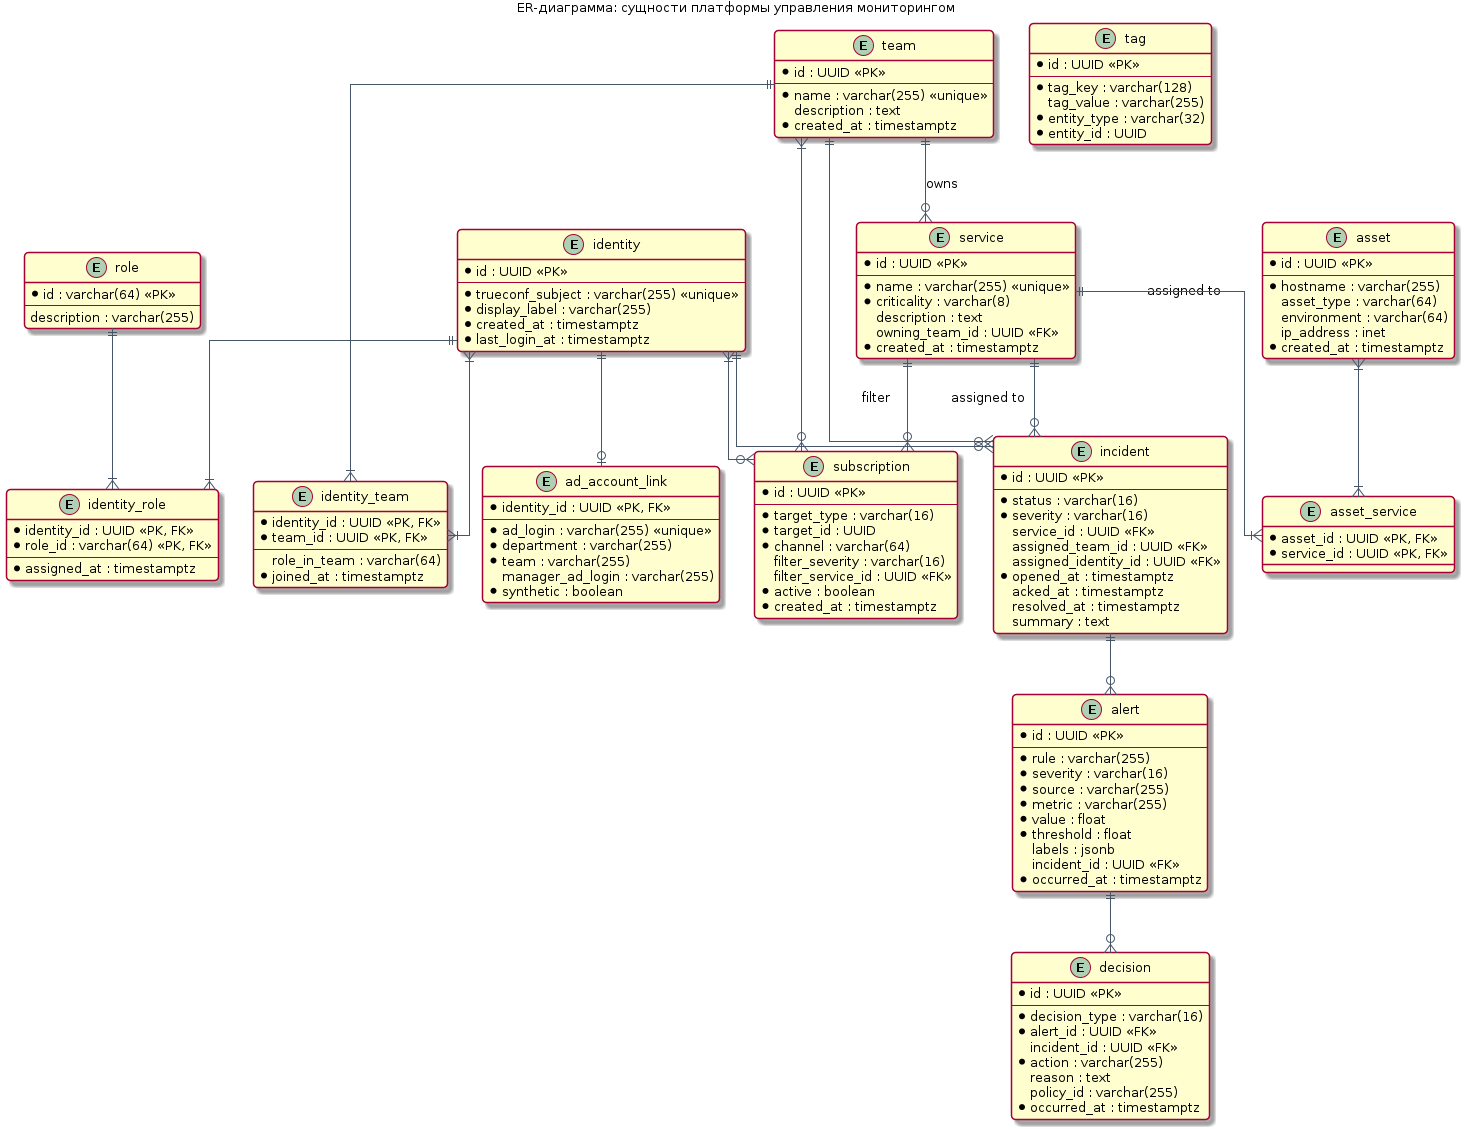
\includegraphics[width=\textwidth]{img/entity-relationship.png}
    \captionof{figure}{Схема сущностей и связей}
    \label{fig:erd}
\end{figure}


\end{document}
%%% Local Variables:
%%% mode: latex
%%% TeX-master: t
%%% End:
